%%%%%%%%%%%%%%%%%%%%%%%%%%%%%%%%%%%%%%%%%%%%%%%%%%%%%%%%%%%%%%%%%%%%%%%%
\chapter{Approximate Maximum Weighted Matching in Dynamic Networks}
\label{ch:dyn-mwm}
% Labels: approximate, dynamic, static
%%%%%%%%%%%%%%%%%%%%%%%%%%%%%%%%%%%%%%%%%%%%%%%%%%%%%%%%%%%%%%%%%%%%%%%%

\section{Introduction}

\paragraph{Context}
Given a graph $G = (V, E, w)$, a matching $M \subseteq E$ is a set of pairwise
non-adjacent edges,
\ie all the vertices in $G$ are incident to at most one edges in $M$. A
matching is called \emph{maximal} if no edge can be added to it without
violating the matching property. It is called \emph{maximum}, in turn, if there
is no other matching with higher cardinality.
Computing the maximum cardinality matching (MCM) of a graph can be done in
$\Oh(m\sqrt{n})$ time in general graphs by Micali and
Vazirani~\cite{DBLP:conf/focs/MicaliV80} and in $\Oh(n^\omega)$ time in planar graph
with the algorithm by Mucha and
Sankowski~\cite{DBLP:journals/algorithmica/MuchaS06}.\footnote{Recall that
$\omega < \numprint{2.373}$ is the matrix multiplication exponent.}

On weighted graphs, the maximum weighted matching (MWM) is the matching
with maximum edge weight -- the edge weight of a matching $M$ is the sum
of the weights of the edges in $M$. \change{The fastest known algorithms
for this problem are by Gabow~\cite{DBLP:conf/soda/Gabow90}, which takes
$\Oh(nm + n^2\log n)$ time, and by Galil~\cite{galil1986efficient}, which}
takes $\Oh(mn\log n)$.
Assuming integral edge weights, Gabow and Tarjan~\cite{DBLP:journals/jacm/GabowT91}
require $\Oh(m\sqrt{n}\log(nW))$ time, where $W$ is the highest edge weight,
while Sankowski~\cite{DBLP:journals/tcs/Sankowski09} (by restricting the input to
bipartite graphs) requires $\tilde{\Oh}(Wn^\omega)$ time, where $\tilde{\Oh}$
hides a polylogarithmic factor. For a broader overview of matching algorithms,
we refer the reader to
Refs.~\cite{bisseling2020parallel,lawler2001combinatorial,lovasz2009matching}.

\paragraph{Motivation}
Computing a maximum (weighted) matching  requires superlinear running time and
is thus impractical on today's large real-world graph datasets. To mitigate
long running times, it is common to resort to approximation. Preis's greedy
algorithm~\cite{DBLP:conf/stacs/Preis99} computes a $\change{(1/2)}$-approximation of the
matching with highest weight in $\Oh(m)$ time; the same result is also achieved
with the path-growing algorithm (PGA) by Drake and
Hougardy~\cite{DBLP:conf/wea/DrakeH03}. The main disadvantage of those
algorithms is that they are inherently sequential and thus cannot exploit
parallelism, a common acceleration strategy for massive data.
Birn \etal~\cite{DBLP:conf/europar/BirnOSSS13}, in turn, provide a parallel
implementation of the local max algorithm~\cite{DBLP:journals/corr/cs-DC-0410047},
which computes a maximal matching of an unweighted graph and a $\change{(1/2)}$-approximation
of the MWM of a weighted graph in $\Oh(\log^2 n)$ expected time.
Manne and Halappanavar~\cite{DBLP:conf/ipps/ManneH14} introduced \suitor, a
parallel $\change{(1/2)}$-approximation algorithm based on local domination that
\change{is faster} previous strategies and is amenable to parallelism.

Real-world networks are not only large but often change over time:
edges are inserted, deleted, or change their weight -- see
\Cref{sec:prelim-dynamic-graphs}. Even with a linear-time algorithm,
it would be excessively expensive to compute (or approximate) a maximum (weighted)
matching from scratch every time the graph changes. In recent years,
several fully-dynamic algorithms for both exact and approximate
MCM~\cite{DBLP:conf/icalp/ArarCCSW18,DBLP:journals/jea/BarenboimM19,
DBLP:journals/siamcomp/BaswanaGS18,DBLP:conf/soda/BernsteinS16,
DBLP:journals/siamcomp/BhattacharyaHI18,DBLP:conf/stoc/BhattacharyaHN16,
DBLP:journals/corr/abs-1711-06883,DBLP:conf/soda/0001LSSS19,DBLP:conf/focs/GuptaP13,
DBLP:conf/wg/IvkovicL93,DBLP:journals/ipl/KashyopN20,DBLP:journals/talg/NeimanS16,
DBLP:conf/stoc/OnakR10,DBLP:conf/soda/Sankowski07,DBLP:conf/focs/Solomon16}
and MWM~\cite{DBLP:conf/fsttcs/AnandBGS12,DBLP:conf/focs/GuptaP13,
DBLP:conf/innovations/StubbsW17} have been proposed. These algorithms
perform a static computation of the matching on an initial snapshot
of the graph and exploit this information to update the matching more
efficiently than a static rerun when the graph changes.
Main limitations of existing fully-dynamic algorithms are either
a weaker quality guarantee (\eg Ref.~\cite{DBLP:conf/fsttcs/AnandBGS12}),
or an expensive time complexity (\eg Ref.~\cite{DBLP:conf/focs/GuptaP13}).
To the best of our knowledge, none of the existing algorithms for
fully-dynamic MWM support batch updates and the only existing implementation
is provided in Ref.~\cite{conf/acda/AngrimanMSU21}.

\paragraph{Contribution}
In this chapter, we introduce a new algorithm that takes inspiration
from \suitor~\cite{DBLP:conf/ipps/ManneH14} and maintains a
$\change{(1/2)}$-approximation of the MWM in fully-dynamic graphs. The main idea
is simple: we use the static \suitor algorithm to compute an approximate
MWM on an initial snapshot of the graph. Then, after an edge update,
our dynamic algorithm identifies the affected vertices (\ie those
whose matching partner needs to be updated) and updates the matching
accordingly.

Our implementation also supports multiple edge insertions or removals in
batches. For
single edge updates, our dynamic algorithm has a worst-case time complexity
of $\Oh(n + m)$, whereas for batches with $b$ edge updates it is
$\Oh(b\cdot(n + m))$. Although this does not improve the static time complexity,
our dynamic algorithm performs remarkably well in practice: \change{i}n our experiments,
we evaluate its running time on real-world (complex and road) and synthetic
networks with up to $\numprint{2.5}$ billion edges. Our results show that,
compared to the best algorithm presented in Ref.~\cite{conf/acda/AngrimanMSU21},
our dynamic \suitor algorithm handles single graph updates faster and yields
matchings with at most \quaRWMaxDrop lower weight.
Concerning batch updates, in comparison to a static recomputation (for lack of
another meaningful MWM baseline in this setting), our algorithm can handle
batches of $10^4$ of such updates $10^2\times$ to $10^3\times$ faster.
%
Furthermore, the time required by our dynamic algorithm for every considered
batch size is always below a millisecond. Thus, our algorithm's implementation
provides real-time capabilities even without parallelism.

\bibnotes{My contributions among those in this chapter involve
the new dynamic algorithms and proofs, part of the implementation work,
carrying out the experiments, and the presentation of the results. Preliminary
work and experiments on dynamic algorithms for MWM were conducted by Micha{\l}
Boro{\'n} under the supervision of Henning Meyerhenke. The contributions of
this chapter are also joint work with Micha{\l} Boro{\'n} and Henning
Meyerhenke and are currently in revision for international journal
publication.}

\section{Preliminaries}
\subsection{Problem Definition and Notation}
Let $G = (V, E, w)$ be a simple undirected graph with positive edge weights.
A matching in $G$ is a subset of pairwise non-adjacent edges $M \subseteq E$ --
alternatively, one can see a matching as a subgraph of $G$ (restricted to the
edges) with degree at most 1. A vertex is \emph{matched} if it is incident
to an edge in $M$, otherwise it is called \emph{unmatched} or \emph{free}.

In the maximum-weight matching problem (MWM), the objective is to compute
a matching $M^\star$  that maximizes the sum of the edge weights.

\begin{cproblem}{Maximum-weight Matching}
\begin{tabular}{ll}
\textbf{Input:} & Undirected weighted graph $G = (V, E, w)$.\\
\textbf{Find:} & Matching $M^\star$ s.t. $\sum_{e \in M^\star}w(e)$ is maximal.
\end{tabular}
\end{cproblem}

In the context of fully-dynamic graphs, if an edge update\footnote{Recall that
by \enquote{edge update} we mean either an edge insertion, an edge removal, or
an edge weight change.} happens to $G$, we denote by $G' = (V, E', w')$ the
graph after the edge update. Similarly, we denote by $N'(u)$ the set of
neighbors of a vertex $u$ in $G'$. Given a matching $M$ computed on $G$ and a
sequence of graph updates, our objective is to update $M$ in $G'$ faster (in
terms of empirical running time) than recomputing a new matching in $G'$ from
scratch, while retaining the theoretical bound on the solution quality.

\subsection{Related Work}
\label{sec:dyn-mwm:related-work}

In the following, we summarize relevant works concerning MCM and MWM in both
static and dynamic settings.

\paragraph{Static Algorithms}
Edmond's blossom algorithm~\cite{edmonds1965paths} (time complexity: $\Oh(mn^2)$)
and the later improved algorithm by Micali and Vazirani~\cite{DBLP:conf/focs/MicaliV80}
($\Oh(m\sqrt{n})$ time) are two popular strategies to compute an MCM
based on augmenting paths. Goldberg and Karzanov~\cite{DBLP:journals/mp/GoldbergK04}
propose a blocking skew-symmetric flow algorithm that achieves the same running time
as Micali and Vazirani. More recent works use data reduction
rules~\cite{DBLP:conf/esa/KorenweinNNZ18} or shrink-tree data
structures~\cite{DBLP:conf/alenex/DroschinskyMT20} to achieve better running times
in practice on sparse real-world networks.
%
If we restrict the input to planar graphs, the randomized algorithm by
Mucha and Sankowski~\cite{DBLP:journals/algorithmica/MuchaS06} computes
an MCM in $\Oh(n^\omega)$ time via Gaussian elimination.

Concerning the MWM problem, Galil~\cite{galil1986efficient} provides
the fastest known algorithm, which takes $\Oh(mn\log n)$ time.
Assuming integral edge weights, the algorithm by Duan
\etal~\cite{DBLP:journals/talg/DuanPS18} takes $\Oh(m\sqrt{n}\log(nW))$
time, improving over Gabow and Tarjan's algorithm~\cite{DBLP:journals/jacm/GabowT91}.
The latter takes $\tilde{\Oh}(\log(nW))$ time, where $\tilde{\Oh}$ hides
a polylogarithmic factor and $W$ is the highest edge weight. On bipartite
graphs, Sankowski~\cite{DBLP:journals/tcs/Sankowski09} requires
\change{$\tilde{O}(Wn^\omega)$} time.

Running a superlinear algorithm is often too expensive on large graphs.
Therefore, several approximation algorithms with (nearly-)linear running
time have been introduced.
A naive greedy algorithm that iteratively adds to the matching
the (heaviest) edge that does not violate the matching condition
takes $\Oh(m\log n)$ time and achieves a $\change{(1/2)}$-approximation
for both the MCM and MWM problems~\cite{DBLP:journals/networks/Avis83}.
Preis~\cite{DBLP:conf/stacs/Preis99} reduced the running time to $\Oh(m)$
while retaining the same quality guarantee. Further strategies to obtain
the $1/2$ bound are the one by Manne and Bisseling~\cite{DBLP:conf/ppam/ManneB07}
based on dominant edges, the local max algorithm investigated by Birn
\etal~\cite{DBLP:conf/europar/BirnOSSS13}, the path growing algorithms by
Drake and Hougardy~\cite{DBLP:conf/wea/DrakeH03,DBLP:journals/ipl/DrakeH03},
the global paths algorithm by Maue and Sanders~\cite{DBLP:conf/wea/MaueS07},
and \suitor by Manne and Halappanavar~\cite{DBLP:conf/ipps/ManneH14}.

\paragraph{Dynamic Algorithms}
A trivial strategy maintains a $\change{(1/2)}$-approximation of a maximal
matching on dynamic graphs in $\Oh(n)$ time per update by resolving
all augmenting paths of length one.
This result has been improved in several works.
The update time was reduced for the first time to $\Oh((n + m)^{\sqrt{2}/2})$
by Ivkovi\'c and Lloyd~\cite{DBLP:conf/wg/IvkovicL93}. The randomized algorithm
by Onak and Rubinfeld~\cite{DBLP:conf/stoc/OnakR10} maintains a $\Oh(1)$-approximation
of an MCM in $\Oh(\log^2 n)$ expected amortized update time; this result was further
improved by Baswana \etal~\cite{DBLP:journals/siamcomp/BaswanaGS18}, who reduced the
update time to $\Oh(\log n)$ and the approximation ratio to $1/2$.
Sol\change{o}mon~\cite{DBLP:conf/focs/Solomon16} further reduced the amortized
update time of Baswana \etal from logarithmic to constant.
%
Deterministic algorithms for approximate MCM have been presented first by
Bhattacharya \etal~\cite{DBLP:conf/stoc/BhattacharyaHN16}, who maintain a
$(3 + \epsilon)$-approximate MCM in $\tilde{\Oh}(\min(\sqrt{n}, m^{1/3}/\epsilon))$
amortized update time; the update time was later reduced to constant but at the
cost of a weaker $\Oh(1)$-approximation
guarantee~\cite{DBLP:journals/siamcomp/BhattacharyaHI18}.
In terms of worst-case bounds for MCM, the best known algorithms are the ones
from Gupta and Peng~\cite{DBLP:conf/focs/GuptaP13} (which maintains a $(1 +
\epsilon)$-approximation with $\Oh(\sqrt{m}/\epsilon)$ update time), Neiman
and Solomon~\cite{DBLP:journals/talg/NeimanS16} (which maintains a $3/2$-approximation
with $\Oh(\sqrt{m})$ update time), and Bernstein and Stein~\cite{DBLP:conf/soda/BernsteinS16}
(which maintains a $(3/2 + \epsilon)$-approximation with $\Oh(m^{1/4}\cdot\epsilon^{-\numprint{2.5}})$
update time).
The first $(2 + \epsilon)$-approximation algorithms in $\Oh(\text{poly}\log n)$ update time
were introduced independently by Charikar and
Solomon~\cite{DBLP:journals/corr/abs-1711-06883} and by Arar
\etal~\cite{DBLP:conf/icalp/ArarCCSW18}, whereas Grandoni
\etal~\cite{DBLP:conf/soda/0001LSSS19} gave a $(1 + \epsilon)$-approximation algorithm in
the incremental setting requiring a constant amortized update time. For graphs
with constant neighborhood independence, Barenboim and
Maimon~\cite{DBLP:journals/jea/BarenboimM19} present an algorithm for MCM with
deterministic $\tilde{\Oh}(n)$ update time. For lax and eager algorithms, \ie
two subclasses of fully-dynamic algorithms for maintaining an MCM, Kashyop and
Narayanaswamy~\cite{DBLP:journals/ipl/KashyopN20} prove a conditional lower
bound for the update time that is sublinear in the number of edges.

Despite the vast variety of algorithms for dynamic MCM, very little effort
has been invested in implementing them and evaluating their practical performance
on real-world instances. Only recently, Henzinger \etal~\cite{DBLP:conf/esa/Henzinger0P020}
evaluated dynamic algorithms for MCM in practice. These are the algorithms by
Baswana \etal~\cite{DBLP:journals/siamcomp/BaswanaGS18} ($2$-approximate MCM in
$\Oh(\sqrt{n})$ update time), by Neiman and Solomon~\cite{DBLP:journals/talg/NeimanS16}
($3/2$-approximate MCM in $\Oh(\sqrt{m})$ update time), and two novel algorithms:
one based on random walks and one that uses a depth-bounded blossom algorithm to
find augmenting paths. Their experimental evaluation shows that (i) the optimal
matching can be maintained more than $10\times$ faster than a naive static
recomputation, (ii) the considered approximation algorithms are multiple orders
of magnitude faster than a naive static recomputation, and (iii) the
extended random-walk based algorithms achieve the best practical performance.

Concerning the dynamic MWM problem, Anand \etal~\cite{DBLP:conf/fsttcs/AnandBGS12}
propose a fully-dynamic algorithm for maintaining an $8$-MWM with an expected
amortized time of $\Oh(\log n\log\mathcal{C})$ per edge update, where $\mathcal{C}$
is the ratio between the maximum and the minimum edge weights of the graph.
They also show that the approximation ratio can be reduced to
$\numprint{4.9108}$ without sacrificing performance by using geometric rounding.
Gupta and Peng~\cite{DBLP:conf/focs/GuptaP13} maintain a $(1 + \epsilon)$-approximation
in $\Oh(m^{1/2}\cdot\epsilon^{-2-\Oh(1/\epsilon)}\log W)$ update time in graphs with edge
weights between $1$ and $W$; their strategy runs the static algorithm from time to time,
trims the graph into smaller equivalent graphs whenever possible and partitions the
edges into geometrically shrinking intervals depending on their weights.
%
Stubbs and Williams~\cite{DBLP:conf/innovations/StubbsW17} present metatheorems to
show that, if there exists an $\alpha$-approximation algorithm for MCM with update time
$T$, then there also exists a $2\alpha(1 + \epsilon)$-approximation algorithm for MWM with
$\Oh(T\cdot\epsilon^{-2}\log^2 W)$ update time, where $W$ is the maximum edge
weight. The main idea relies on improving and extending the algorithm by Crouch
and Stubbs~\cite{DBLP:conf/approx/CrouchS14}, who addressed the dynamic MWM problem
in the semi-streaming model. None of the aforementioned algorithms for MWM has been
implemented.
%
For the semi-streaming model, Ghaffari and Wajc~\cite{DBLP:conf/soda/GhaffariW19}
describe a single-pass MWM algorithm with a $(2 + \epsilon)$-approximation ratio
requiring $\Oh(n \log n)$ bits, improving previous
results~\cite{DBLP:conf/approx/CrouchS14,DBLP:journals/siamdm/EpsteinLMS11,
DBLP:journals/tcs/FeigenbaumKMSZ05,DBLP:conf/approx/McGregor05,DBLP:journals/talg/PazS19}.
Again, as in the MCM case, only a few of these algorithms have recently been
implemented~\cite{conf/acda/AngrimanMSU21}.
Ref.~\cite{conf/acda/AngrimanMSU21} provides an experimental
evaluation of dynamic algorithms for MWM inspired by the ones by Maue and
Sanders~\cite{DBLP:conf/wea/MaueS07} and by Stubbs and
Williams~\cite{DBLP:conf/innovations/StubbsW17}.
Experimental data indicate that the approach by Maue and
Sanders~\cite{DBLP:conf/wea/MaueS07} -- which combines random walks with
dynamic programming to find augmenting paths --
yields the best results in terms of running time and quality.
Hereafter, as done in Ref.~\cite{conf/acda/AngrimanMSU21},
we call this algorithm \dynmwmrandom.


\subsection{The Static \suitor Algorithm}
\label{sec:dyn-mwm:static-suitor}
%
Since our dynamic algorithm is built on top of the static one called
\suitor~\cite{DBLP:conf/ipps/ManneH14}, for self-containment purposes
we provide in the following a brief overview of this latter algorithm.

Recall that $w$ is the weight function of the edge. By convention, if
$\set{u, v} \notin E$, or if a vertex reference $v$ is \nil, then
$w(\change{u}, v)$ is $0$. To guarantee a correct execution, we assume that all
vertices in the graph are indexed from $1$ to $n$; in addition, the following
total ordering of the edges incident to the same vertex $u$ is enforced: if
$\set{u, x}$ and $\set{u, y}$ have the same edge weight and $x < y$, than
$w(u, x) < w(u, y)$. During the course of the algorithm, \suitor keeps two
references for each vertex $u \in V$: $\mate(u)$ and $\vsuitor(u)$.
When the execution is finished, $\mate(u)$ refers to the matching partner
of $u$ or is \nil if $u$ remains unmatched. The crucial condition
for selecting a matching partner is given by:

\begin{equation}
\label{eq:mate}
\begin{split}
\mate(u) = \argmax_{v \in N(u)}\{&w(u, v) : \nexists x\in N(v)\ \text{s.t.}\\
                                   &\mate(x) = v \wedge w(x, v) > w(u, v)\}.
\end{split}
\end{equation}

In other words, $v = \mate(u)$ is the neighbor of $u$ for which there is no other neighbor
$x$ of $v$ \enquote{pointing} to $v$ with $\set{u, x}$ dominating $\set{u, v}$.
If no such vertex exists, $\mate(u)$ is set to \nil (\ie $u$ is unmatched).

\begin{algorithm}[tb]
\caption{Recursive \findsuitor function}
\label{algo:rec-find-suitor}
\begin{algorithmic}[1]
\Function{findSuitor}{$u$}
\State$\mate(u) \gets \argmax_{v \in N(u)}\set{w(u, v) : w(u, v) > w(v, suitor(v)}$
\If{$p(u) \neq \nil$}
\State$y \gets \vsuitor(\mate(u))$
\State$\vsuitor(\mate(u)) \gets u$
\If{$y \neq \nil$}
\State$\textsc{findSuitor}(y)$
\EndIf
\EndIf
\EndFunction
\end{algorithmic}
\end{algorithm}

\begin{algorithm}[tb]
\caption{Static recursive \suitor algorithm~\cite{DBLP:conf/ipps/ManneH14}}
\label{algo:rec-suitor}
\textbf{Input:} Undirected graph $G = (V, E, w)$\\
\textbf{Output:} $\change{(1/2)}$-approximation of the MWM of $G$

\begin{algorithmic}[1]
\For{\textbf{each} $u \in V$}
\State$\mate(u) \gets \nil$
\State$\vsuitor(u) \gets \nil$
\EndFor
\For{\textbf{each} $u \in V$}\label{line:rec-suitor:find-suitor-for}
\State$\textsc{findSuitor}(u)$\Comment{\Cref{algo:rec-find-suitor}}
\EndFor
\end{algorithmic}
\end{algorithm}



\Cref{algo:rec-suitor} shows the pseudocode of the \suitor algorithm: $\mate$
and $\vsuitor$ are initially set to \nil for every vertex in the graph; then,
the recursive function \findsuitor (\Cref{algo:rec-find-suitor}) sets $\mate$
according to \Cref{eq:mate} for every vertex. The progress of the algorithm can
be described in the following Lemma:

\begin{lemma}[\cite{DBLP:conf/ipps/ManneH14}, Lemma 3.2]
Following \change{each} call to \findsuitor in \Cref{algo:rec-suitor} from the loop over
the vertices of $G$, $\mate(u)$ is set according to \Cref{eq:mate} for each vertex
$u$ processed so far.
\end{lemma}

Clearly, after the execution of \Cref{algo:rec-suitor}, the condition in \Cref{eq:mate}
is true for all vertices and this leads us to the next property of the resulting matching:

\begin{lemma}[\cite{DBLP:conf/ipps/ManneH14}, Lemma 3.1]
\label{lemma:dyn-mwm:mate-greedy}
If $\mate(u)$ is set according to \Cref{eq:mate} for each vertex $u \in V$, then
$\mate(\cdot)$ defines the same matching as the greedy algorithm.
\end{lemma}

\begin{proof}
See Ref.~\cite[Section 3.2]{DBLP:journals/siamsc/KhanPPSSMHD16}. The proof is
for $b$-matching, but contains the MWM problem by setting $b$ to $1$.
\end{proof}

\begin{algorithm}[t]
\caption{\footnotesize Iterative \findsuitor function}
\label{algo:iter-find-suitor}
\begin{algorithmic}[1]
\footnotesize
\Function{findSuitor}{$u$}
\State$\cur \gets u$
\State$\done \gets \false$
\Repeat
\State$\partner \gets \vsuitor(\cur)$
\State$\heaviest \gets ws(\cur)$
\For{\textbf{each} $v \in N(\cur)$}\label{line:iter-find-suitor:for-neigh}
\If{$w(\cur, v) > \heaviest$ \textbf{and} $w(\cur, v) > ws(v)$}
\State$\partner \gets v$
\State$\heaviest \gets w(\cur, v)$
\EndIf
\EndFor\label{line:iter-find-suitor:for-neigh-end}
\State$\done \gets \true$
\If{$\heaviest > 0$}\label{line:iter-find-suitor:if-heaviest}
\State$y \gets \vsuitor(\partner)$\label{line:iter-find-suitor:update-1}
\State$\vsuitor(\partner) \gets \cur$
\State$ws(\partner) \gets \heaviest$\label{line:iter-find-suitor:update-2}
\If{$y \neq \nil$}\label{line:iter-find-suitor:if-y}
\State$\cur \gets y$
\State$\done \gets \false$\label{line:iter-find-suitor:if-y-end}
\EndIf
\EndIf
\Until{$\done$ is \true}
\EndFunction
\end{algorithmic}
\end{algorithm}

\begin{algorithm}[t]
\footnotesize
\caption{\footnotesize Static iterative \suitor algorithm~\cite{DBLP:conf/ipps/ManneH14}}
\label{algo:iter-suitor}
\textbf{Input:} Undirected graph $G = (V, E, w)$\\
\textbf{Output:} $\change{(1/2)}$-approximation of the MWM of $G$

\begin{algorithmic}[1]
\For{\textbf{each} $u \in V$}
\State$\vsuitor(u) \gets \nil$
\State$ws(u) \gets 0$
\EndFor
\For{\textbf{each} $u \in V$}
\State$\textsc{findSuitor}(u)$\Comment{\Cref{algo:iter-find-suitor}}
\EndFor
\end{algorithmic}
\end{algorithm}


Thus, regardless of the order in which the \texttt{for}-loop
(\Cref{line:rec-suitor:find-suitor-for}, \Cref{algo:rec-suitor}) processes the
vertices, \suitor is a deterministic algorithm that computes the same matching
as the well-known greedy algorithm that adds permissible edges in the order of
decreasing weight. Due to our assumption of a total edge ordering, this matching
is unique.

\Cref{algo:iter-suitor} shows the iterative version of \suitor, which does not
use $\mate$ any more but only $\vsuitor$. An additional array $ws$ stores the
value $w(u, suitor(u))$ for each vertex $u \in V$. We rewrite the condition
in \Cref{eq:mate} in terms of $\vsuitor$ as follows:

\begin{equation}
\label{eq:suitor}
\begin{split}
    suitor(u) = \argmax_{v \in N(u)}\{&w(u, v) : \nexists y \in N(v)\ \text{s.t.}\\
                                      &suitor(v) = y \wedge w(y, v) > w(u, v)\}.
\end{split}
\end{equation}

If no such vertex exists, $\vsuitor(u)$ is \nil. Similarly to its recursive
counterpart, for every vertex $u\in V$, \Cref{algo:iter-suitor} initializes
$\vsuitor$ and $ws$ to \nil and $0$, respectively, and calls the iterative
function $\findsuitor(u)$ (\Cref{algo:iter-find-suitor}). \findsuitor uses a
variable \cur to store the vertex that is seeking a new partner in the current
iteration -- \ie a vertex $u$ in the recursive \findsuitor.
In \Crefrange{line:iter-find-suitor:for-neigh}{line:iter-find-suitor:for-neigh-end},
it determines whether there exists a neighbor $v$ of \cur and, if so, it stores
$v$ and $w(cur, v)$ into the \partner and \heaviest variables, respectively.
In \Cref{line:iter-find-suitor:if-heaviest}, if \heaviest is $0$, no such neighbor
exists and the function terminates because \done is left to \true -- hence,
\cur remains unmatched. Otherwise, \partner was set to the matching partner of
\cur and \heaviest to $w(\cur, \partner)$; in
\Crefrange{line:iter-find-suitor:update-1}{line:iter-find-suitor:update-2}, $y$
stores the previous matching partner of \partner (if any) before making \cur the
new matching partner of \partner by setting $\vsuitor(\partner)$ to \cur and
$ws(\partner)$ to \heaviest. Then, in
\Crefrange{line:iter-find-suitor:if-y}{line:iter-find-suitor:if-y-end}, if $y$ is
not \nil, then \partner had a previous potential matching partner $y$; therefore $y$
needs to seek a new potential matching partner and this is done by setting \cur to
$y$ and \done to \false\ -- which is equivalent to a recursive call of
\Cref{algo:rec-find-suitor}.

\section{Dynamic \suitor Algorithm for Single Edge Updates}
\label{sec:dyn-mwm:dyn-suitor-single}
%
In this section, we first describe how we extend the static \suitor algorithm to
also handle single edge updates. Building upon that, we generalize our approach
to multiple edge updates in batches in \Cref{sec:dyn-mwm:multiple-edge-updates}.

We index variables of the \suitor algorithm with the superscript \interm
(for intermediate) [or \final for final, resp.] if they refer to the state directly
after the edge change [or after the dynamic \suitor algorithm has been run], \eg
$\vsuitor\interm(u)$ [or $\vsuitor\final(u)$].
The matching $M\interm$ as well as other \suitor variables are derived from $M$
(and the other counterparts) by taking the edge update on $G$ into account.
For example, if an edge $e$ is deleted from $G$ that is part of $M$, then
$M\interm = M\setminus\set{e}$. Our goal is to update/improve the intermediate
matching $M\interm$ efficiently, \ie to avoid redundant computations when computing
the final matching $M\final$. We will show that $M\final$ equals the matching $M'$
computed by the static \suitor algorithm on $G'$. To this end, we define the notion
of \emph{affected} vertex.

\begin{definition}
\label{def:dyn-mwm:affected-vertices}
A vertex $u$ is called \emph{affected} iff $M\interm$ violates \Cref{eq:suitor} for
$\vsuitor\interm(u)$, \ie iff:

\[
\vsuitor\interm(u) \neq \argmax_{v \in N'(u)}\{w'(u, v) : \nexists y\in N'(v)\ \text{s.t.}
\ \vsuitor\interm(v) = y \wedge w'(y, v) > w'(u, v)\}.
\]
\end{definition}

\begin{algorithm}[t]
\footnotesize
\caption{\footnotesize
Extended version of the \findsuitor function (\Cref{algo:iter-find-suitor}) that finds the affected
vertices}
\label{algo:dyn-suitor-find-aff}
\textbf{Input:} Affected vertex $z$\\
\textbf{Output:} Stack of affected vertices

\begin{algorithmic}[1]
\Function{findAffected}{$z$}
\State$S_A \gets$ empty stack
\State$\cur \gets z$
\State$\done \gets \false$
\Repeat
\State$\partner \gets \vsuitor(\cur)$
\State$\heaviest \gets ws(\cur)$
\For{\textbf{each} $x \in N(\cur)$}\label{line:dyn-find-affected:for-neighbors}
\If{\textbf{not} $\affected(x)$ \textbf{and} $w(\cur, x) > \heaviest$ \textbf{and} $w(\cur, x) > ws(x)$}
\label{line:dyn-find-suitor:first-if}
\State$\partner \gets x$
\State$\heaviest \gets w(\cur, x)$
\EndIf
\EndFor
\State$\done \gets \true$
\If{$\heaviest > ws(\partner)$}\label{line:dyn-find-affected:if-heaviest}
\State$y \gets \vsuitor(\partner)$
\State$\vsuitor(\partner) \gets \cur$\label{line:dyn-find-suitor:update-1}
\State$ws(\partner) \gets \heaviest$\label{line:dyn-find-suitor:update-2}
\State$S_A.\texttt{push}(\partner)$\label{line:dyn-find-suitor:sa-push}
\State$\affected(\partner) \gets \true$
\If{$y \neq \nil$}\label{line:dyn-find-affected:if-y}
\State$\vsuitor(y) \gets \nil$\label{line:dyn-find-suitor:inv-1}
\State$ws(y) \gets 0$\label{line:dyn-find-suitor:inv-2}
\State$\affected(y) \gets \true$
\State$\cur \gets y$
\State$\done \gets \false$
\EndIf
\Else
\State$\affected(\cur) \gets \false$\label{line:dyn-find-affected:mark-unaffected}
\EndIf
\Until{$\done$ is \true}
\State\Return$S_A$
\EndFunction
\end{algorithmic}
\end{algorithm}

\begin{algorithm}[t]
\footnotesize
\caption{\footnotesize Updates \vsuitor and $ws$ of the matching partners of the
vertices into the stack $S_A$}
\label{algo:dyn-suitor-update-aff}
\textbf{Input:} Stack of affected vertices $S_A$

\begin{algorithmic}[1]
\While{$S_A$ is not empty}
\State$x \gets S_A.\texttt{pop}()$
\State$y \gets \vsuitor(x)$
\State$\vsuitor(y) \gets x$\label{line:dyn-mwm:update-aff-1}
\State$ws(y) \gets ws(x)$\label{line:dyn-mwm:update-aff-2}
\State$\affected(x) \gets \false$\label{line:dyn-mwm:update-aff-unaff-1}
\State$\affected(y) \gets \false$\label{line:dyn-mwm:update-aff-unaff-2}
\EndWhile
\end{algorithmic}
\end{algorithm}


Our dynamic algorithm computes $M\final$ after an edge update by finding all the vertices
affected by the edge update (\findaff function in \Cref{algo:dyn-suitor-find-aff}) and by
then updating their matching partner so that \Cref{eq:suitor} is satisfied
(\updateaff function in \Cref{algo:dyn-suitor-update-aff}). If \Cref{eq:suitor} is
satisfied for every vertex in $G'$, it follows from \Cref{lemma:dyn-mwm:mate-greedy}
that the resulting matching is (the unique) $M'$.

The \findaff function (\Cref{algo:dyn-suitor-find-aff}) is an extended version
of the \findsuitor function (\Cref{algo:iter-find-suitor}) used by the
iterative \suitor algorithm; it uses a boolean array \affected to keep track of
the affected vertices and pushes the affected vertices whose \vsuitor and $ws$
variables need to be updated onto a stack $S_A$.
%
As in \findsuitor, \cur is the vertex we are trying to find a new matching
partner for, \partner is the preferred matching partner for \cur\ -- \ie the
vertex that satisfies \Cref{eq:suitor} for \cur, if any -- and $\heaviest =
w'(\cur, \partner)$.
%
Then, in \Crefrange{line:dyn-find-suitor:update-1}{line:dyn-find-suitor:update-2},
if a new matching partner for \cur is found, the $\vsuitor\final(\partner)$
and $ws\final(\partner)$ variables are updated to \cur and \heaviest, respectively;
additionally, \partner is pushed onto $S_A$ (\Cref{line:dyn-find-suitor:sa-push}).
If \partner is matched in $M$ with another vertex $y$, then the edge
$\set{\partner, y}$ would violate the matching condition and this needs to be
removed from the matching; this is done in
\Crefrange{line:dyn-find-suitor:inv-1}{line:dyn-find-suitor:inv-2}
by \enquote{invalidating} the vertex $y$, \ie setting the values of
$\vsuitor\final(y)$ and $ws\final(y)$ to \nil and $0$, respectively.
As in \findsuitor, in the next iteration we seek for a new partner for the
invalidated vertex $y$ by updating \cur to $y$.
%
This procedure is repeated until either a new partner for \cur
cannot be found (\ie \cur is free in $M'$), or \partner is free in $M$.
By keeping track of the affected vertices, we guarantee that a previously
invalidated vertex is not selected as new matching partner in future iterations
of the loop (see \Cref{line:dyn-find-suitor:first-if}).

The stack $S_A$ is later used by \updateaff (\Cref{algo:dyn-suitor-update-aff})
to match the affected vertices that were not updated by \findaff (\ie the ones
that were stored in the \cur variable) to their new partner
(\Crefrange{line:dyn-mwm:update-aff-1}{line:dyn-mwm:update-aff-2}).
Once a pair of matched vertices has eventually been processed,
they are not affected anymore and thus \updateaff marks them as unaffected
(\Crefrange{line:dyn-mwm:update-aff-unaff-1}{line:dyn-mwm:update-aff-unaff-2}).
In the following, we show how these two functions are used in case of an edge insertion
or an edge removal and that our dynamic algorithm yields a matching $M\final$
that equals the matching $M'$ computed by the static \suitor algorithm on $G'$.
Concerning edge weight updates, they can be handled as an edge removal followed
by an edge insertion.

\subsection{Edge Insertions}
\label{sec:dyn-mwm:single-insertions}
%
Let us first address the case in which an edge is inserted into $G$, \ie $G' =
(V, E, \cup \set{u, v})$ with $e = \set{u, v} \notin E$. Intuitively, this new
edge will only be part of the new matching $M'$ iff it is \enquote{a better
deal} for both $u$ and $v$. In other words: $e \in M'$ iff $w'(u, v)$ is
heavier than both $w'(u, \vsuitor\interm(u))$ and $w(v, \vsuitor\interm(v))$
and is thus the dominant edge for both. We show this in the following lemma:

\begin{lemma}
\label{lemma:dyn-mwm:affected-insertion}
Let $G' = (V, E\cup e)$ with $e = \set{u, v} \notin E$.\\
Then: $e\in M' \Leftrightarrow w'(u, v) > \max\set{w(u, \vsuitor\interm(u)), w(v, \vsuitor\interm(v))}$.
\end{lemma}

\begin{proof}
We develop the proof \wilog for $u$ by assuming that $w(u, \vsuitor\interm(u))
> w(v, \vsuitor\interm(v))$; the proof for $v$ is symmetric. Let $Y \subseteq
N(u)$ be the set of vertices $y$ that do not have any neighbor $x$ such that
$w(x, y) > \max\{w(x, \vsuitor\interm(x)), w(u, y)\}$, \ie the set of vertices
among which \Cref{eq:suitor} selects $\vsuitor(u)$ as the vertex $y$ with
maximum $w(y, u)$. We also define $Y^{(v)} := Y \cup \set{v}$.

\enquote{$\Rightarrow$}:
From $e\in M'$ we have that $\vsuitor'(v) = u$, and from \Cref{eq:suitor} it
follows that $v = \argmax_{y \in Y^{(v)}}w'(u, y)$. Therefore, since
$\vsuitor\interm(u) \in Y^{(v)}$, $w'(u, v) > w'(u, \vsuitor\interm(u))$.

\enquote{$\Leftarrow$}:
By definition, we have that $\vsuitor\interm(u) = \argmax_{y \in Y}w'(u, y)$
and that $\vsuitor'(u) = \argmax_{y \in Y^{(v)}}w'(u, y)$. By hypothesis,
$w'(u, v) > w(u, \vsuitor\interm(u))$, and thus $\vsuitor'(u) = \argmax_{y \in
Y^{(v)}}w'(u, y) = v$. The same holds if we exchange $u$ and $v$ in the
argument. Therefore, $e \in M'$.
\end{proof}

\begin{algorithm}[t]
\footnotesize
\caption{\footnotesize Dynamic \suitor algorithm for single edge insertions}
\label{algo:dyn-suitor-single-ins}
\textbf{Input:} Graph $G' = (V, E \cup \set{u, v}, w')$, an edge $\set{u, v} \notin E$

\begin{algorithmic}[1]
\If{$w'(u, v) > \max\{w'(u, \vsuitor\interm(u)), w'(v, \vsuitor\interm(u))\}$}
\label{line:dyn-suitor-single-ins:check-affected}
\State$\affected(x) \gets \false\ \forall x\in V$
\For{$z \in \set{v, u}$}
\State$\affected(z) \gets \true$
\State$S_A \gets \textsc{findAffected}(z)$
\State$\textsc{updateAffected}(S_A \setminus \{\vsuitor\interm(z)\})$
\label{line:dyn-suitor-single-ins:upd-aff}
\EndFor
\EndIf
\end{algorithmic}
\end{algorithm}


\Cref{algo:dyn-suitor-single-ins} shows our dynamic algorithm for single edge
insertions.
In
\Cref{line:dyn-suitor-single-ins:check-affected}, given a newly added edge
$e = \set{u, v}$, the algorithm excludes $e$ if it does not satisfy
\Cref{lemma:dyn-mwm:affected-insertion} because $e$ is then also not part of $M'$.
As we will show later, all the vertices affected by an edge insertion lie on
two alternating paths that start from $u$ and $v$ and that alternate edges in
$M'\setminus M$ with edges in $M\setminus M'$, as shown in \Cref{fig:dyn-mwm:edge-insertion}.
In the \texttt{for}-loop, our algorithm finds the affected
vertices that lie on these two alternating paths and updates their matching partner
according to \Cref{eq:suitor}.
This is done as follows: the first vertex in the path is marked as affected,
\findaff updates the $\vsuitor$ and $ws$ variables of the
affected $\partner$ vertices and pushes them onto a stack $S_A$. Finally, \updateaff
matches the vertices in $S_A$ to their new partner.
Note that, in \Cref{line:dyn-suitor-single-ins:upd-aff}, $\vsuitor\interm(z)$
is removed from $S_A$ to avoid overwriting $\vsuitor(z)$ in \updateaff;
this information is needed in the next iteration of the for loop to find the
affected vertices in the alternating path that starts from $u$.

We now analyze in more detail which vertices are affected by the insertion of
an edge $e = \set{u, v} \notin E$ that satisfies
\Cref{lemma:dyn-mwm:affected-insertion} (and is thus in $M'$) and how $M\final$
is computed starting from $M\interm$. In the following, we split our analysis
into three possible scenarios: both $u$ and $v$ are unmatched (Case 1), only
one of $u$ and $v$ is matched (Case 2), and both $u$ and $v$ are matched (Case
3).

\begin{figure}[tb]
\centering
\begin{subfigure}[t]{.485\textwidth}
\centering
\begin{tikzpicture}[scale=.7]
\small

\coordinate (u) at (0, 1);
\coordinate (v) at (0, -1);
\coordinate (x1) at (1.5, 2);
\coordinate (y1) at (1.5, -2);
\coordinate (x2) at (3, 2);
\coordinate (y2) at (3, -2);
\coordinate (x3) at (4.5, 1);
\coordinate (y3) at (4.5, -1);
\coordinate (x4) at (6, 1);
\coordinate (x5) at (7.5, 2);
\filledvertex{u}
\filledvertex{v}

\foreach \i in {1,...,5} {
    \filledvertex{x\i}
    \draw (x\i) node [above = 3pt] {$x_\i$};
}

\draw (u) node [left = 3pt] {$u$};
\draw (v) node [left = 3pt] {$v$};

\edge{u}{v}
\dashedEdge{u}{x1}
\edge{x1}{x2}
\dashedEdge{x2}{x3}
\edge{x3}{x4}
\dashedEdge{x4}{x5}

\end{tikzpicture}

\caption{The affected vertices are covered by one alternating
path $P_v$.}
\label{fig:dyn-mwm:edge-insertion-pv}
\end{subfigure}\hfill
\begin{subfigure}[t]{.485\textwidth}
\begin{tikzpicture}[scale=.8]
\small

\coordinate (u) at (0, 1);
\coordinate (v) at (0, -1);
\coordinate (x1) at (1.5, 2);
\coordinate (y1) at (1.5, -2);
\coordinate (x2) at (3, 2);
\coordinate (y2) at (3, -2);
\coordinate (x3) at (4.5, 1);
\coordinate (y3) at (4.5, -1);
\coordinate (x4) at (6, 1);
\coordinate (y4) at (6, -1);
\coordinate (x5) at (7.5, 2);
\filledvertex{u}
\filledvertex{v}

\foreach \i in {1,...,5} {
    \filledvertex{x\i}
    \draw (x\i) node [above = 3pt] {$x_\i$};
}
\foreach \i in {1,...,4} {
    \filledvertex{y\i}
    \draw (y\i) node [below = 3pt] {$y_\i$};
}

\draw (u) node [left = 3pt] {$u$};
\draw (v) node [left = 3pt] {$v$};

\edge{u}{v}
\dashedEdge{u}{x1}
\dashedEdge{v}{y1}
\edge{x1}{x2}
\edge{y1}{y2}
\dashedEdge{x2}{x3}
\dashedEdge{y2}{y3}
\edge{x3}{x4}
\edge{y3}{y4}
\dashedEdge{x4}{x5}

\end{tikzpicture}

\caption{The affected vertices are covered by two alternating paths
$P_u$ and $P_v$.}
\label{fig:dyn-mwm:edge-insertion-pu-pv}
\end{subfigure}

\caption{Examples of alternating paths that cover the vertices affected by the insertion
of an edge $\set{u, v}$.
Solid lines and dashed lines represent edges in $M'\setminus M$ and edges in $M\setminus M'$,
respectively.
In \Cref{fig:dyn-mwm:edge-insertion-pv} there is only one
alternating path because $u$ is matched in $M$ and $v$ is not, whereas
in \Cref{fig:dyn-mwm:edge-insertion-pu-pv} there are two because both $u$ and
$v$ are matched in $M$.}
\label{fig:dyn-mwm:edge-insertion}
\end{figure}

\subsubsection{Case 1: $u$ and $v$ both unmatched}
%
Let us first cover the trivial case where both $u$ and $v$ are unmatched in $M$, \ie
there is no vertex in $G$ that satisfies \Cref{eq:suitor} for both $u$ and $v$.
In the following Lemma, we show that $M' = M\interm\cup \set{e}$ and that $u$
and $v$ are the only affected vertices.

\begin{lemma}
\label{lemma:dyn-mwm:insert-case-1}
Let $e = \set{u, v} \notin E$. If both $u$ and $v$ are unmatched in $M$, then
$M' = M \cup \set{e}$ and $u$ and $v$ are the only affected vertices.
\end{lemma}

\begin{proof}
The proof is symmetric for $u$ and $v$, we develop it for $u$.
If $u$ is unmatched in $M$, then $\vsuitor\interm(u) = \nil$ and there
is no neighbor of $u$ that satisfies \Cref{eq:suitor} in $G$.
After the insertion of $e$ we have that $0 = w'(u, \vsuitor\interm(u)) < w'(u,
v)$ and thus $v$ satisfies \Cref{eq:suitor} for $u$.
Further, all the neighbors of $u$ in $G$ are already matched,
and matching $u$ with $v$ cannot invalidate \Cref{eq:suitor} for any of them.
Therefore, $M' = M\interm \cup \set{e}$ and no other vertex apart from $u$ and
$v$ is affected.
\end{proof}

We now show that $M\final$ equals $M'$, \ie \Cref{eq:suitor} is fulfilled by
$M\final$ for every vertex in $G'$. The condition in
\Cref{line:dyn-suitor-single-ins:check-affected} in
\Cref{algo:dyn-suitor-single-ins} is clearly true because both $u$ and $v$ are
free. In $\findaff(v)$, we have that $\cur = v$ and $\partner = u$. Thus,
$\vsuitor\final(u)$ is set to $v$ and $u$ is pushed onto $S_A$. $\findaff(v)$
performs only one iteration since $y = \vsuitor\interm(u) = \nil$ and
$\updateaff$ has no effect since its input stack is empty. The next iteration
of the for loop performs the same operations but with $u$ and $v$ swapped.
Thus, the resulting matching is $M\final = M\interm\cup\set{e} = M'$.

\subsubsection{Case 2: $u$ matched and $v$ unmatched}
To analyze the case where just one of $u$ and $v$ is matched in $M$, our
analysis assumes \wilog that $u$ is matched in $M$ and $v$ is not; the other
case is symmetric. We first describe how \Cref{algo:dyn-suitor-single-ins}
identifies all the affected vertices and then how it updates their matching
partner.

In this scenario, $u$ and $v$ are not the only vertices affected by the
insertion of $e$ because \Cref{eq:suitor} is violated also for
$\vsuitor\interm(u)$. In particular, we show in
\Cref{lemma:dyn-mwm:alternating-path} that the vertices affected by the
insertion of $e$ are covered by a simple (\ie without loops) path that,
starting from $v$, alternates edges in $M'\setminus M$ with edges in
$M\setminus M'$ as shown in~\Cref{fig:dyn-mwm:edge-insertion-pv}. We show this
in the following lemma.

\begin{lemma}
\label{lemma:dyn-mwm:alternating-path}
Let $e = \set{u, v} \notin E$ be a newly inserted edge such that $e \in M'$.
If $u$ is matched in $M$ and $v$ is not, then all the vertices affected by the
insertion of $e$ are connected by a simple alternating path $P_v$
that starts from $v$ and that alternates edges in $M'\setminus M$ with edges in
$M\setminus M'$. Further, the weights of the edges along $P_v$ are decreasing,
\ie for each $e_1, e_2\in P_v$ where $e_1$ precedes $e_2$ in $P_v$, we have
that $w'(e_1) > w'(e_2)$.
\end{lemma}

\begin{proof}
Clearly, $e \in M' \setminus M$ is the first edge in $P_v$. As shown in
\Cref{fig:dyn-mwm:edge-insertion-pv}, let $x_1 = \vsuitor\interm(u)$: $e \in
M'$ implies that \Cref{eq:suitor} is violated for $x_1$ in $G'$. If no vertex
$x_2\in N'(x_1)$ satisfies~\Cref{eq:suitor} for $x_1$, then $x_1$ remains
unmatched in $M'$ and no further vertex is affected. Otherwise, there exists
another vertex $x_2\in N'(x_1)$ that satisfies~\Cref{eq:suitor} for $x_1$. In
the former case, the alternating path has only two edges: $e$ and $e_1 =
\set{u, x_1}\in M\setminus M'$. In the latter case, $\vsuitor\final(x_1) = x_2$
and $\vsuitor\final(x_2) = x_1$. Hence, in addition to $e_1$, the alternating
path has at least another edge $e_2 = \set{x_1, x_2}\in M'\setminus M$. By
repeating with $e_1$ the same logic we applied to $e$, it follows that the
vertices affected by the insertion of $e$ lie on a path $P_u$ that, starting
from $u$, follows edges in $M'$ and in $M$ alternately.

What's left to be shown is that $P_v$ is simple, which can be done similarly as
in the final part of the proof of~\cite[Lemma 3.2]{DBLP:conf/ipps/ManneH14}.
Note that, if $x_1$ is affected, then $w'(u, x_1) < w'(u, \vsuitor\final(u) =
v)$ and $w'(x_1, \vsuitor\final(x_1) = x_2) < w'(u, x_1)$, and thus $w'(x_1,
\vsuitor\final(x_1)) < w'(u, \vsuitor\final(u))$. In words, the weights of the
edges along $P_v$ are decreasing because every time an affected vertex $x_1$
loses its matching partner $\vsuitor\interm(x_1)$, it holds: if it finds a new
partner $\vsuitor\final(x_1) = x_2$, then $w'(x_1, x_2)$ must be smaller than
$w'(x_1, \vsuitor\interm(x_1))$. Therefore, it is not possible for $x_1$ to be
matched in $M'$ with a vertex that is already covered by $P_v$, which implies
that $P_v$ is simple.
\end{proof}

Note that, as shown in \Cref{fig:dyn-mwm:edge-insertion-pv}, the alternating
path $P_v = (u, v, x_1, \ldots, x_\ell)$ alternates vertices $x_i$ that are
matched in $M'$ with a \enquote{worse partner} (in terms of edge weight) than
the one they had in $M$ (\ie the ones where $i$ is odd), and vertices $x_i$
that are matched in $M'$ with a \enquote{better partner} than the one they had
in $M$ (\ie $u$, $v$, and the ones where $i$ is even). Hereafter, we will call
the former ones \enquote{downgraded} and the latter ones \enquote{upgraded}.
More formally:

\begin{lemma}
\label{lemma:dyn-mwm:alternating-path-upgr-downgr}
For each vertex $x_i$ in an alternating path $P_v = (v, u, x_1, \ldots,
x_\ell)$, for each $1 \leq i \leq \ell$ it holds: if $i$ is odd, then $w'(x_i,
\vsuitor\final(x_i)) < w'(x_i, \vsuitor\interm(x_i))$ (\ie $x_i$ is
downgraded); otherwise, $i$ is even and $w'(x_i, \vsuitor\final(x_i)) > w'(x_i,
\vsuitor\interm(x_i))$ (\ie $x_i$ is upgraded).
\end{lemma}

\begin{proof}
Every downgraded vertex $x_i$ loses its initial matching partner
$\vsuitor\interm(x_i)$ because $\vsuitor\interm(x_i)$ is matched in $M'$ with
another (upgraded) vertex -- \eg $x_1$ loses its initial matching partner $u$
because $\set{u, v}\in M'$. Note that, in $P_v$, the upgraded vertex matched
with $\vsuitor\interm(x_i)$ in $M'$ comes always earlier than $x_i$; from
\Cref{lemma:dyn-mwm:alternating-path} we know that the weights of the edges
along $P_v$ are decreasing, and thus $w'(x_i, \vsuitor\interm(x_i)) < w'(x_i,
\vsuitor\final(x_i))$. Further, by construction of the alternating path, $P_v$
alternates downgraded and upgraded vertices from $x_1$ on. Thus, knowing that
$x_1$ is downgraded, all the remaining $x_i$ with odd $i$ are also downgraded.

If $x_i$ is upgraded, it is either one of $u$ and $v$, or it is
$\vsuitor\final(x_{i - 1})$ of the previous downgraded vertex $x_{i - 1}$ in
$P_v$. Since by our hypothesis $x_i$ is in $P_v$, we also have that
$\vsuitor\final(x_i) = x_{i - 1}$, hence $w'(x_i, \vsuitor\final(x_i) = x_{i -
1}) > w'(x_i, \vsuitor\interm(x_i))$.
\end{proof}

\begin{remark}
\label{lemma:alt-path-upg-downg-uniq}
Due to the total ordering of the edge weights,
the alternating path $P_v$ is unique and can be computed deterministically as
the sequence of the vertices stored in the $cur$ and $partner$
variables of the $\findsuitor(v)$ function (\Cref{algo:iter-find-suitor}).
\end{remark}

From \Cref{lemma:dyn-mwm:alternating-path} it follows that, to compute $M'$, we need
to find the affected vertices in the alternating path $P_v$ and update their
$\vsuitor\final$ and $ws\final$ values according to \Cref{eq:suitor}. In the
following we show that \Cref{algo:dyn-suitor-single-ins} finds all the vertices
in $P_v$ and updates their matching partner according to \Cref{eq:suitor},
so that $M\final$ equals $M'$.


\begin{proposition}
\label{prop:dyn-mwm:find-aff-correctness}
The $\findaff(v)$ function (\Cref{algo:dyn-suitor-find-aff}) computes
$\vsuitor\final$ and $ws\final$ according to \Cref{eq:suitor} for the upgraded
vertices in $P_v$ and pushes them onto a stack $S_A$.
\end{proposition}
%
\begin{proof}
The function maintains the following loop invariant:
$\cur$ is either $v$ or an invalidated downgraded vertex $x_i \in P_v$;
in the first case, $\partner$ is $u$; in the second case, if the condition in
\Cref{line:dyn-find-affected:if-heaviest} is true, then $\partner$ is an improving
vertex $x_{i + 1} \in P_v$ -- otherwise both the loop and $P_v$ stop.
Maintaining the invariant guarantees that $\findaff(v)$ covers all affected vertices in $P_v$
and that all the improving vertices $x_i$ are updated according to \Cref{eq:suitor}
and pushed onto $S_A$.

The invariant obviously holds in the first two iterations.
In the first one, we have that $\cur = v$,
$\partner = u$, and $y = \vsuitor\interm(u) = x_1$
(see \Cref{fig:dyn-mwm:edge-insertion-pv}). In the next one, $\cur = x_1$ is invalidated from
the previous iteration, and thus it is a downgraded vertex in $P_v$
that is seeking a new partner to replace the previous partner $u$;
if a new partner $x_2$ is found, $\partner = x_2$ is an upgraded vertex in
$P_v$, thus $\vsuitor\final(x_2)$ and $ws\final(x_2)$
are updated to $x_1$ and $w'(x_1, x_2)$,
respectively, and it is pushed onto $S_A$
(\Crefrange{line:dyn-find-suitor:update-1}{line:dyn-find-suitor:sa-push}).
By applying the same logic to the remaining vertices in $P_v$,
the invariant also holds for the remaining iterations of $\findaff(v)$.
We remark that, by marking the vertices in $P_v$ as affected, the function cannot
iterate on the same vertices multiple times.
The function terminates when either $\partner$ is a free vertex (hence $y
= \nil$), or there is no neighbor of $\cur$ that satisfies \Cref{eq:suitor}, and
thus $\cur$ remains unmatched in $M\final$.
\end{proof}

Note that, if $P_v$ ends with a downgraded (hence free) vertex $x_\ell$, $\findaff(v)$
invalidates it before terminating, \ie $\vsuitor\final(x_\ell)$ and $ws\final(x_\ell)$ are updated
according to \Cref{eq:suitor}. Therefore, $x_\ell$ is not affected anymore in $G'$ and
thus marked as unaffected (\Cref{line:dyn-find-affected:mark-unaffected}).

\begin{proposition}
After \updateaff finishes, all vertices in $P_v$ satisfy \Cref{eq:suitor} in $G'$.
\end{proposition}

\begin{proof}
From \Cref{prop:dyn-mwm:find-aff-correctness} we know that, when \updateaff is
called, all the upgraded vertices satisfy \Cref{eq:suitor} in $G'$ and that
they are stored in the stack $S_A$. \updateaff \enquote{completes} the matching
$M\final$ by updating, for all the downgraded vertices $x_i\in P_v$ matched in
$M'$, their $\vsuitor\final(x_i)$ and $ws\final(x_i)$ values to $x_{i + 1}$ and
$w'(x_i, x_{i + 1})$, respectively, and thus all vertices in $P_v$ satisfy
\Cref{eq:suitor} in $G'$.
\end{proof}


\begin{proposition}
\label{prop:dyn-mwm:edge-insertion-time}
If $u$ is matched in $M$ and $v$ is not (or vice versa),
\Cref{algo:dyn-suitor-single-ins} has a worst-case running time
that is linear in the number of the affected vertices and in
the sum of their degrees.
\end{proposition}

\begin{proof}
\Cref{algo:dyn-suitor-single-ins} invokes \findaff and \updateaff twice. The
number of iterations of \findaff is linear in the length of a simple
alternating path that covers the vertices
affected by the edge insertion (\Cref{lemma:dyn-mwm:alternating-path}). In each
iteration, \findaff iterates over all the neighbors of the current vertex
(\Cref{line:dyn-find-affected:for-neighbors}) and all the other operations have
constant time complexity.

\updateaff performs constant-time operations on each vertex in $S_A$.
\findaff pushes at most one vertex onto $S_A$ in each iteration, and thus
the worst-case time complexity of \updateaff is linear in the number of
affected vertices.
\end{proof}

\begin{remark}
\label{remark:dyn-mwm:run-time-single-insertion}
In the worst case, all vertices in the graph are affected by an edge insertion
and then \findaff performs at most $n$ iterations and visits all edges twice.
Therefore, the worst-case time complexity of \Cref{algo:dyn-suitor-single-ins}
is $\Oh(n + m)$.
\end{remark}


\subsubsection{Case 3: $u$ and $v$ both matched}
%
To settle the final case, we show (i) that the affected vertices are
covered by two alternating paths $P_v$ and $P_u$ and then (ii)
that the matching $M\final$ computed by \Cref{algo:dyn-suitor-single-ins} equals $M'$.

\begin{lemma}
\label{lemma:dyn-mwm:alternating-paths}
Let $\set{u, v}\notin E$ be a newly inserted edge such that $e \in M'$. If both $u$ and $v$
are matched in $M$, then all the vertices affected by the insertion of $e$ are connected
by two simple alternating paths $P_v$ and $P_u$ with decreasing edge weights
that start from $v$ and $u$, respectively, and that alternate edges in $M'
\setminus M$ and edges in $M\setminus M'$.
\end{lemma}

\begin{proof}
We proceed similarly as in \Cref{lemma:dyn-mwm:alternating-path}. As shown in
\Cref{fig:dyn-mwm:edge-insertion-pu-pv}, $e\in M'\setminus M$ is the first edge for
both $P_v$ and $P_u$. Thus, \Cref{eq:suitor} is violated for both
$x_1  = \vsuitor\interm(u)$ and $y_1 = \vsuitor\interm(v)$ (due to the
matching condition, $x_1 \neq y_1$). Consequently, the edges
$e_{1, u} = \set{u, x_1}$ and $e_{1, v} = \set{v, y_1}$ are removed from
$M\interm$, which implies that $e_{1,u}, e_{1, v} \in M
\setminus M'$. Now let $x_2$ and $y_2$ be the two
vertices (if any) that satisfy \Cref{eq:suitor} for $x_1$ and $y_1$,
respectively, in $G'$.
Clearly, we have that $\set{x_1, x_2}, \set{y_1, y_2} \in M' \setminus M$. If
$x_2$ and/or $y_2$ are matched in $M$, then we can apply recursively to
their matching partners the same logic as we did with $x_1$ and $y_1$.
Hence, $P_v$ and $P_u$ are constructed exactly as described in
\Cref{lemma:dyn-mwm:alternating-path} and thus they are both simple and have
decreasing edge weights.
\end{proof}

In the following, we show that the vertices along $P_v$ and $P_u$ are computed
in the two iterations of \Cref{algo:dyn-suitor-single-ins}.
A crucial observation is that our dynamic algorithm computes one alternating
path at a time -- $P_u$ is computed after $P_v$.
Therefore, when a new $\partner$ vertex for $\cur$ is found while computing $P_v$
(\ie in $\findaff(v)$), this might not be the actual vertex that satisfies
\Cref{eq:suitor} for $\cur$ in $G'$ because it is computed without
considering the affected vertices in $P_u$ -- they are yet to be computed.
If this is the case, then it results in a wrong computation of $P_v$ and thus,
immediately after the first iteration of \Cref{algo:dyn-suitor-single-ins},
some of the vertices covered by $\findaff(v)$ are in a \enquote{wrong state}, \ie
\Cref{eq:suitor} is locally satisfied for them but not for all the vertices in $G'$.
However, we show later that, in this case, the second iteration of
\Cref{algo:dyn-suitor-single-ins} not only updates the affected vertices in $P_u$,
but also corrects the vertices that are in a wrong state, so that eventually all
vertices in $G'$ fulfill \Cref{eq:suitor} and thus $M\final = M'$. For this
purpose, we expand our notation by denoting the values of the variables of
\suitor and $P_v$ immediately after the first iteration of
\Cref{algo:dyn-suitor-single-ins} with superscript $\iinterm$.

Clearly, if in $P_v\iinterm$ there are no vertices in a wrong state, then
$P_v\iinterm = P_v$ and $P_u$ is computed exactly in the same way as $P_v$ (as
in Case 2) and no further analysis is
required. Otherwise, the two paths intersect: let $y_i$ be the last vertex in
$P_u$ before $P_u$ intersects $P_v\iinterm$ and let $x_j$ be the vertex in
$P_v\iinterm$ adjacent to $y_i$ (\eg vertices $x_5$ and $y_5$ in
\Cref{fig:dyn-mwm:intersect-2}). We observe that an intersection always happens when
$\findaff(u)$ selects a vertex in $P_v\iinterm$ as new matching partner for the
current vertex $y_i$ in $P_u$. Therefore, $y_i$ is always a downgraded vertex
and $x_j$ satisfies \Cref{eq:suitor} for $y_i$ in $G'$. Depending on the
position of $x_j$ in $P_v\iinterm$, we identify three possible subcases and treat
them separately: (i) $x_j$ is downgraded and it is the last vertex in
$P_v\iinterm$ (as in \Cref{fig:dyn-mwm:intersect-2}), (ii) $x_j$ is downgraded and
internal in $P_v\iinterm$ (as in \Cref{fig:dyn-mwm:intersect-3}), and (iii) $x_j$ is
upgraded (as in \Cref{fig:dyn-mwm:intersect-4}).

\begin{figure}[tb]
\centering
\begin{subfigure}[t]{.49\textwidth}
\centering
\begin{tikzpicture}[scale=.7]
\small

\coordinate (u) at (0, 1);
\coordinate (v) at (0, -1);
\coordinate (x1) at (1.5, 2);
\coordinate (y1) at (1.5, -2);
\coordinate (x2) at (3, 2);
\coordinate (y2) at (3, -2);
\coordinate (x3) at (4.5, 1);
\coordinate (y3) at (4.5, -1);
\coordinate (x4) at (6, 1);
\coordinate (x5) at (7.5, 2);
\filledvertex{u}
\filledvertex{v}

\foreach \i in {1,...,5} {
    \filledvertex{x\i}
    \draw (x\i) node [above = 3pt] {$x_\i$};
}

\draw (u) node [left = 3pt] {$u$};
\draw (v) node [left = 3pt] {$v$};

%\draw[-] (u) -- (v) node [midway, right = 3pt] {$e$};
%\draw[dashed] (u) -- (y) node [midway, below right = 3pt] {};

\edge{u}{v}
%\dashedEdge{z}{x3}
\dashedEdge{u}{x1}
\edge{x1}{x2}
\dashedEdge{x2}{x3}
\edge{x3}{x4}
\dashedEdge{x4}{x5}

\end{tikzpicture}

\caption{Affected vertices immediately after the computation of $P_v\iinterm$
and before the computation of $P_u$. This represents $M\iinterm$, not
$M\final$ since $P_u$ is yet to be computed.}
\label{fig:dyn-mwm:intersect-1}
\end{subfigure}\hfill
\begin{subfigure}[t]{.49\textwidth}
\centering
\begin{tikzpicture}[scale=.7]
\small

\coordinate (u) at (0, 1);
\coordinate (v) at (0, -1);
\coordinate (x1) at (1.5, 2);
\coordinate (y1) at (1.5, -2);
\coordinate (x2) at (3, 2);
\coordinate (y2) at (3, -2);
\coordinate (x3) at (4.5, 1);
\coordinate (y3) at (4.5, -1);
\coordinate (x4) at (6, 1);
\coordinate (y4) at (6, -1);
\coordinate (x5) at (7.5, 2);
\coordinate (y5) at (7.5, 0);
\filledvertex{u}
\filledvertex{v}

\foreach \i in {1,...,5} {
    \filledvertex{x\i}
    \draw (x\i) node [above = 3pt] {$x_\i$};
    \filledvertex{y\i}
    \draw (y\i) node [below = 3pt] {$y_\i$};
}

\draw (u) node [left = 3pt] {$u$};
\draw (v) node [left = 3pt] {$v$};

\edge{u}{v}
\dashedEdge{u}{x1}
\dashedEdge{v}{y1}
\edge{x1}{x2}
\edge{y1}{y2}
\dashedEdge{x2}{x3}
\dashedEdge{y2}{y3}
\edge{x3}{x4}
\edge{y3}{y4}
\dashedEdge{x4}{x5}
\dashedEdge{y4}{y5}
\edge{x5}{y5}

\end{tikzpicture}

\caption{Case 1: matching $M\final$ after $P_u$ is computed.
The last vertex $x_5$ in $P_v\iinterm$ is free in $M\iinterm$,
$P_u$ intersects $P_v\iinterm$ in $x_5$, and $x_5$ is matched with $y_5$
in $M\final$.}
\label{fig:dyn-mwm:intersect-2}
\end{subfigure}

\begin{subfigure}[t]{.49\textwidth}
\centering
\begin{tikzpicture}[scale=.7]
\small

\coordinate (u) at (0, 1);
\coordinate (v) at (0, -1);
\coordinate (x1) at (1.5, 2);
\coordinate (y1) at (1.5, -2);
\coordinate (x2) at (3, 2);
\coordinate (y2) at (3, -2);
\coordinate (x3) at (4.5, 1);
\coordinate (y3) at (4.5, -1);
\coordinate (x4) at (6, 1);
\coordinate (x5) at (7.5, 2);
\filledvertex{u}
\filledvertex{v}

\foreach \i in {1,...,5} {
    \filledvertex{x\i}
    \draw (x\i) node [above = 3pt] {$x_\i$};
}
\foreach \i in {1,...,3} {
    \filledvertex{y\i}
    \draw (y\i) node [below = 3pt] {$y_\i$};
}

\draw (u) node [left = 3pt] {$u$};
\draw (v) node [left = 3pt] {$v$};

\edge{u}{v}
\dashedEdge{u}{x1}
\dashedEdge{v}{y1}
\edge{x1}{x2}
\edge{y1}{y2}
\dashedEdge{x2}{x3}
\dottedEdge{x3}{x4}
\dashedEdge{y2}{y3}
\edge{y3}{x3}
\dashdottedEdge{x4}{x5}

\end{tikzpicture}


\caption{Case 2: matching $M\final$ after $P_u$
is computed. $P_u$ intersects $P_v\iinterm$ in $x_3$, which is
internal in $P_v\iinterm$.
$P_v\iinterm$ from $x_4$ on is undone.}
\label{fig:dyn-mwm:intersect-3}
\end{subfigure}\hfill
\begin{subfigure}[t]{.49\textwidth}
\centering
\begin{tikzpicture}[scale=.7]
\small

\coordinate (u) at (0, 1);
\coordinate (v) at (0, -1);
\coordinate (x1) at (1.5, 2);
\coordinate (y1) at (1.5, -2);
\coordinate (x2) at (3, 2);
\coordinate (y2) at (3, -2);
\coordinate (x3) at (4.5, 1);
\coordinate (y3) at (4.5, -1);
\coordinate (x4) at (6, 1);
\coordinate (x5) at (7.5, 2);
\coordinate (z4) at (6, -1);
\coordinate (z5) at (7.5, 0);
\filledvertex{u}
\filledvertex{v}

\foreach \i in {1,...,5} {
    \filledvertex{x\i}
    \draw (x\i) node [above = 3pt] {$x_\i$};
}
\foreach \i in {1,...,3} {
    \filledvertex{y\i}
    \draw (y\i) node [below = 3pt] {$y_\i$};
}

\foreach \i in {4, 5} {
    \filledvertex{z\i}
    \draw (z\i) node [above = 3pt] {$z_\i$};
}


\draw (u) node [left = 3pt] {$u$};
\draw (v) node [left = 3pt] {$v$};

\edge{u}{v}
\dashedEdge{u}{x1}
\dashedEdge{v}{y1}
\edge{x1}{x2}
\edge{y1}{y2}
\dashedEdge{x2}{x3}
\dashedEdge{y2}{y3}
\dottedEdge{x3}{x4}
\edge{y3}{x4}
\dashedEdge{x4}{x5}

\draw (x3) edge[dash dot,out=270, in=180] (z4);
\dottedEdge{z4}{z5}

\end{tikzpicture}

\caption{Case 3: matching $M\final$ after $P_u$ is computed.
$P_u$ intersects $P_v\iinterm$ in $x_4$ which is upgrade and
continues with $x_3$.}
\label{fig:dyn-mwm:intersect-4}
\end{subfigure}

\caption{Examples of intersecting alternating paths computed by \Cref{algo:dyn-suitor-single-ins}
to update the matching after the insertion of an edge $\set{u, v}$.
\Cref{fig:dyn-mwm:intersect-1} shows the status of the affected vertices after the
computation of $P_v\iinterm$ and before the computation of $P_u$.
\Crefrange{fig:dyn-mwm:intersect-2}{fig:dyn-mwm:intersect-4} show the three possible
cases of intersection between $P_v\iinterm$ and $P_u$.
Dashed and solid edges have the same meaning as in \Cref{fig:dyn-mwm:edge-insertion}, dotted edges
are in $M\iinterm\setminus M\final$, dash-dotted edges are in $M\final \setminus M\iinterm$.}

\label{fig:dyn-mwm:edge-insertion-intersect}
\end{figure}

\paragraph{Subcase (i) -- $x_j$ is downgraded and it is the last vertex in $P_v\iinterm$}
%
In this case (see \Cref{fig:dyn-mwm:intersect-2}), $x_j$ is free in $M\iinterm$ because
$suitor\iinterm(y_i) = y_{i - 1}$ and no other vertex in $N'(x_j)$ satisfies
the condition in \Cref{line:dyn-find-suitor:first-if} of $\findaff(v)$
for $x_j$. Hence, $x_j$ is in a wrong state because it is not
matched with $y_i$, its actual matching partner in $M'$.
The wrong state of $x_j$ is corrected by $\findaff(u)$: when $P_u$ reaches
$y_i$, $\vsuitor\final(x_j)$ and $ws\final(x_j)$ are set to $y_i$ and
$w'(x_j, y_i)$, respectively. Also, $x_j$ is pushed onto $S_A$,
so that $y_i$ will eventually be matched with $x_j$ in \updateaff.

\paragraph{Subcase (ii) -- $x_j$ is downgraded and it is internal in $P_u$}
%
Here, $x_j$ is in a wrong state for the same reason as in subcase (i).
The main difference (see \Cref{fig:dyn-mwm:intersect-3})
is that $P_v\iinterm$ does not finish in $x_j$ because there exists
a vertex $\partner = x_{j + 1} \in N'(x_j)$ that satisfies the conditions in
\Cref{line:dyn-find-suitor:first-if,line:dyn-find-affected:if-heaviest} in $\findaff(v)$.
Thus, all the vertices in $P_v\iinterm$ after $x_j$ are in a wrong state as well,
because they are not affected, but their matching partner is updated
by \Cref{algo:dyn-suitor-single-ins}. However, in the following lemma we show
that the second iteration of the algorithm matches $x_j$ to its matching
partner in $M'$ and restores the original matching partners of the vertices in
$P_v\iinterm$ after $x_j$.

\begin{lemma}
The second iteration of \Cref{algo:dyn-suitor-single-ins} matches $x_j$ with
its matching partner in $M'$ and restores the original matching partners of the
vertices in $P_v\iinterm$ after $x_j$.
\end{lemma}
%
\begin{proof}
As in case (i), $x_j$ fulfills \Cref{eq:suitor}
for $y_i$ and once $\findaff(u)$ reaches $y_i$ it matches $x_j$ to $y_i$.
%
Recall that the vertices in $P_v\iinterm$
after $x_j$ are in a wrong state in $M\iinterm$, because their matching
has been updated, although they are not affected by the edge insertion.
Hence, we need to show that for these vertices, $\findaff(u)$
restores the matching partner they have in $M$ -- \ie the same
as in $M'$ since they are not affected.

Let $x_{j + 1}$ be $\change{\vsuitor\interm(x_j)}$; in the iteration where $\partner$
is $x_j$, $\findaff(u)$ keeps iterating with $\cur = x_{j + 1}$. Hereafter,
$\findaff(u)$ maintains the following invariant: $\cur$ is an upgraded vertex
in $\change{M\interm}$ and, if $\heaviest > ws\iinterm(\partner)$, then $\partner$ is
the matching partner of $\cur$ in $M$; otherwise $\cur$ is free in $M'$.
%
Due to the properties of the alternating path we have that, in $\change{M\interm}$,
$x_{j + 1}$ is an upgraded vertex, because it is matched with $x_j$ and
$w'(x_j, x_{j + 1}) > w'(x_{j + 1}, x_{j + 2})$. In $M'$, in turn, we have that
$x_{j + 1}$ is either free or matched with another vertex $x_{j + 2}$. In the
first case, $\findaff(u)$ stops at $x_{j + 1}$ and leaves it unmatched, because
there is no other vertex in $N'(x_{\change{i} + 1})$ that satisfies \Cref{eq:suitor}.
Otherwise, we need to show that $\findaff(u)$ selects $x_{j + 2}$ as matching
partner for $x_{j + 1}$.
%
From \Cref{lemma:dyn-mwm:alternating-paths}, the vertices on $P_v\iinterm$ and
$P_u$ before $x_{j + 1}$ satisfy \Cref{eq:suitor} and thus cannot be selected
as partners for $x_{j + 1}$. Furthermore, $x_{j + 2}$ satisfies
\Cref{eq:suitor} for $x_{j + 1}$ in $G'$, and it is downgraded in $M\iinterm$
(hence $w'(x_{j + 2}, \vsuitor\iinterm(x_{j + 2})) < w'(x_{i + 1}, x_{j + 2})$),
which means that the conditions in
\Cref{line:dyn-find-suitor:first-if,line:dyn-find-affected:if-heaviest}
hold. Also, the edge weights are decreasing along $P_v\iinterm$
(\Cref{lemma:dyn-mwm:alternating-paths}),
implying that no other neighbor of $x_{i + 1}$ in $P_v\iinterm$
satisfies \Cref{eq:suitor} for $x_{j + 1}$ in $G'$; hence,
$\set{x_{i + 1}, x_{i + 2}} \in M\final$. The same applies to the remaining
vertices in $P_v\iinterm$.
\end{proof}


\paragraph{Subcase (iii) -- $x_j$ is upgraded.}
In this case (see \Cref{fig:dyn-mwm:intersect-4}), we have that $\set{x_{j-1}, x_j}\in M\iinterm$
and that $w'(y_i, x_j) > w'(x_{j - 1}, x_j) > w'(x_j, x_{j + 1})$.
Thus, $x_{j - 1}$ is in a wrong state because $\set{y_i, x_j}\in M\final$, whereas
the remaining part of $P_v\iinterm$ from $x_j$ on is not necessarily wrong,
because $x_j$ is upgraded also in $P_u$.
$\findaff(u)$ corrects $x_{j - 1}$ by continuing the alternating path from it:
once $\cur = y_i$ is matched with $x_j$, in the next iteration of $\findaff(u)$
we have that $\cur$ is $x_{j - 1}$.
%
Let $z_j$ be the vertex that satisfies \Cref{eq:suitor}
for $x_{j - 1}$ in $G'$ (\eg $z_4$ in \Cref{fig:dyn-mwm:intersect-4}).
If no such vertex exists, then $x_{j - 1}$ is free in $M\final$ and
$\findaff(u)$ stops; otherwise, $P_u$ continues with $z_j$.

We covered now all possible cases that can occur after an edge insertion.
In the following lemma we generalize our results.

\begin{proposition}
\label{prop:dyn-mwm:edge-insertion-time-1}
After an edge insertion, \Cref{algo:dyn-suitor-single-ins} computes
$M'$; its worst-case time complexity is $\Oh(n + m)$.
\end{proposition}

\begin{proof}
The correctness of the resulting matching is shown for every possible case of
edge insertion described in Case 1 to 3. Concerning the worst-case time
complexity, from \Cref{prop:dyn-mwm:edge-insertion-time} and
\Cref{remark:dyn-mwm:run-time-single-insertion} it follows that the first
iteration of \Cref{algo:dyn-suitor-single-ins} has $\Oh(n + m)$ worst-case
running time. The same also holds for the second iteration: due to
\Cref{lemma:dyn-mwm:alternating-paths} $P_u$ is simple, so that its length is
bounded by $\Oh(n)$, and therefore the worst-case time complexity of
\Cref{algo:dyn-suitor-single-ins} is $\Oh(n + m)$.
\end{proof}

Unfortunately, a bound using the number of affected vertices
and their degrees as in \Cref{prop:dyn-mwm:edge-insertion-time} is
\change{difficult to determine} here due to the vertices in a \enquote{wrong}
state.


\subsection{Edge Removals}
\label{sec:dyn-mwm:single-removals}

\begin{algorithm}[t]
\caption{Dynamic \suitor algorithm for single edge removals}
\label{algo:dyn-suitor-single-rem}
\textbf{Input:} Graph $G' = (V, E\setminus \set{u, v}, w')$, an edge $\set{u, v} \in E$

\begin{algorithmic}[1]
\If{$\vsuitor(u) = v$}\label{line:dyn-suitor-rem:rem-condition}
\State$\affected(x) \gets \false\ \forall x \in V$
\State$\vsuitor(u) \gets \nil$\label{line:dyn-suitor-rem:inv-1}
\State$\vsuitor(v) \gets \nil$
\State$ws(u) \gets 0$
\State$ws(v) \gets 0$\label{line:dyn-suitor-rem:inv-2}
\For{$z\in \set{u, v}$}
\State$\affected(z) \gets \true$
\State$S_A \gets \textsc{findAffected}(z)$
\State$\textsc{updateAffected}(S_A)$
\EndFor
\EndIf
\end{algorithmic}
\end{algorithm}


We now address the case in which an edge $\set{u, v} \in E$ is removed from
$G$, \ie $G' = (V, E \setminus \set{u, v})$.

\begin{lemma}
\label{lemma:dyn-mwm:edge-removal}
Let $G' = (V, E \setminus e)$ with $e = \set{u, v} \in E$. Then: $u$ and $v$
are affected $\Leftrightarrow e \in M$.
\end{lemma}

\begin{proof}
We develop the proof \wilog for $u$, for $v$ it is symmetric.

\enquote{$\Leftarrow$}: If $e \in M$, then $u$ is trivially affected since
$\vsuitor\interm(u) = v \notin N'(u)$; $u$ thus violates \Cref{eq:suitor} in
$G'$.

\enquote{$\Rightarrow$}:
Let $Y \subseteq N(u)$ be defined as in
\Cref{lemma:dyn-mwm:affected-insertion}, \ie as the set of neighbors $y$ of $u$
among which \Cref{eq:suitor} selects $\vsuitor(u)$ as the vertex $y$ with
maximum $w(u, y)$. Further, let $Y^{(v)} := Y \setminus \set{v}$. Let us assume
for sake of contradiction that $e \notin M$. Hence, $\vsuitor\interm(u) =
\argmax_{y \in Y} w(u, y) \neq v$ and, in $G'$, this suitor does not change by
having removed $v$ from the neighborhood of $u$. Hence, we have that
$\vsuitor'(u) = \argmax_{y \in Y^{(v)}}w'(u, y) = \vsuitor\interm(u)$, meaning
that $u$ is not affected, which contradicts our hypothesis.
\end{proof}

\Cref{algo:dyn-suitor-single-rem} shows our dynamic algorithm for edge
removals. According to \Cref{lemma:dyn-mwm:edge-removal},
\Cref{line:dyn-suitor-rem:rem-condition} excludes all the removals where the
removed edge $e = \set{u, v}$ is not in $M$. Similarly to edge insertions, we
show later that the vertices affected by an edge removal lie on two alternating
paths that start from $u$ and $v$ and that alternate edges in $M'\setminus M$
with edges in $M\setminus M'$. If $e \in M$, both $u$ and $v$ are affected
downgraded vertices for which we have to find a new partner. First,
\Crefrange{line:dyn-suitor-rem:inv-1}{line:dyn-suitor-rem:inv-2} invalidate
them. Then, as for edge insertions in \Cref{algo:dyn-suitor-single-ins}, the
\texttt{for}-loop uses \findaff to compute the alternating paths of the
affected vertices and to update the matching partner of the upgraded vertices
in the path. Then, it uses \updateaff to update the matching for the downgraded
vertices in the path.

\begin{lemma}
\label{lemma:dyn-mwm:edge-removal-affected}
Let $e = \set{u, v} \in M$. If $e$ is removed from $G$, then all the vertices affected by
the removal of $e$ are connected by two simple alternating paths $P_u$ and $P_v$
with decreasing edge weights that start from $u$ and $v$, respectively, and that
alternate edges in $M'\setminus M$ and edges in $M\setminus M'$.
\end{lemma}

\begin{proof}
As we did in \Cref{lemma:dyn-mwm:alternating-paths}, we need to show that
the construction of $P_u$ and $P_v$ is equivalent to the construction of an
alternating path that connects the vertices affected by an edge insertion as
described in \Cref{lemma:dyn-mwm:alternating-path}.
The only difference is that, after an edge removal, the alternating paths
start from a downgraded vertex rather than from an upgraded vertex.
We develop our proof \wilog for $u$, for $v$ it is symmetric.

Due to \Cref{lemma:dyn-mwm:edge-removal-affected}, $u$ is affected and
downgraded. If there exists a vertex $x_1$ that satisfies \Cref{eq:suitor} for
$u$ in $G'$, then $x_1$ is upgraded and $e_1 = \set{u, x_1} \in M'\setminus
M$; otherwise, $u$ remains free in $G'$ and it is the only vertex in $P_u$.
Similarly, if $x_1$ is matched in $M$ with a vertex $x_2$, then $x_2$ is affected
and downgraded, $e_2 = \set{x_1, x_2} \in M \setminus M'$, and we can apply to
$x_2$ the same logic we applied to $u$; otherwise, $x_1$ is free in $G$ and
$P_u$ has only one edge $e_1$.
Thus, as in \Cref{lemma:dyn-mwm:alternating-path},
the resulting path $P_u$ alternates edges in $M'\setminus M$ and edges in
$M\setminus M'$ as well as downgraded and upgraded vertices.
\end{proof}

Thus, the vertices affected by an edge removal are covered by alternating paths
as the ones shown in \Cref{fig:dyn-mwm:edge-insertion}, with the difference
that the solid lines represent edges in $M\setminus M'$ and the dashed lines
represent edges in $M'\setminus M$.

\begin{proposition}
\label{prop:dyn-mwm:edge-removal-correct}
After \Cref{algo:dyn-suitor-single-rem} finishes, the resulting matching
$M\final$ equals $M'$ in $G'$.
\end{proposition}

\begin{proof}
\Cref{algo:dyn-suitor-single-rem} works analogously to \Cref{algo:dyn-suitor-single-ins},
namely, it uses \findaff and \updateaff to find the affected vertices
along an alternating path and to compute their $\vsuitor\final(\cdot)$ and
$ws\final(\cdot)$. From \Cref{lemma:dyn-mwm:edge-removal-affected} we know that
the vertices affected by an edge removal are covered by two alternating paths
as described in \Cref{lemma:dyn-mwm:alternating-path}.
Thus, the correctness of \Cref{algo:dyn-suitor-single-rem} follows from the
correctness of \Cref{algo:dyn-suitor-single-ins}.
\end{proof}


\begin{proposition}
\label{prop:dyn-mwm:edge-removal-time}
The worst-case running time of \Cref{algo:dyn-suitor-single-rem} is $\Oh(n + m)$.
\end{proposition}

As argued in \Cref{prop:dyn-mwm:edge-removal-correct}, \Cref{algo:dyn-suitor-single-rem}
works analogously to \Cref{algo:dyn-suitor-single-ins}. Thus, they have the
same worst-case time complexity $\Oh(n + m)$ -- see also
\Cref{prop:dyn-mwm:edge-insertion-time-1}.

\section{Extension to Batch Updates}
\label{sec:dyn-mwm:multiple-edge-updates}
%
Our dynamic algorithms for single edge updates can be generalized to batches of
edge updates. The main idea is to run the algorithms for single edge updates
multiple times on the updated graph $G'$. When doing this, we might modify the
$\vsuitor$ and $ws$ variables multiple times. Thus, in this section we use
superscript $\iteri$ to denote the values of these variables after we ran the
algorithm for single edge updates $i$ times. Hence, if the total number of
updates in the batch is $b$, then $^{[b]}$ is equivalent to $\final$.

Note that the crucial difference to an algorithm that updates the matching
after every single edge insertion is that our algorithm runs directly on the
graph $G'$ that already includes a batch $B$ of edge updates.
%
%
Thus, the intermediate matching computed by our algorithm after $i < |B| = b$
iterations is not necessarily the matching that \suitor computes on the initial graph
with the first $i$ edge updates in the batch.
As we explain in
\Cref{sec:dyn-mwm:multiple-insertions,sec:dyn-mwm:multiple-removals}, this
allows our algorithm to update vertices affected by different edge updates in
the same iteration; albeit this does now lower the time complexity, it results
in better practical performances (see \Cref{sec:dyn-mwm:speedups-batch-single}).

\subsection{Multiple Edge Insertions}
\label{sec:dyn-mwm:multiple-insertions}

\begin{algorithm}[t]
\caption{Dynamic \suitor algorithm for a batch of edge insertions}
\label{algo:dyn-suitor-batch-ins}
\textbf{Input:} Graph $G' = (V, E \cup B, w')$, batch of edge insertions
$B = \set{\set{u, v}\ \text{s.t.}\ \set{u, v} \notin E}$

\begin{algorithmic}[1]
\State$\affected \gets \false\ \forall u \in V$
\State$i \gets 0$
\State$\vsuitor\iteri(u) \gets \vsuitor\interm(u)\ \forall u\in V$
\State$ws\iteri(u) \gets ws\interm(u)\ \forall u\in V$
\For{\textbf{each} $\set{u, v} \in B$}\label{line:dyn-suitor-batch-ins:for-ins}
\If{$w'(u, v) > \max\set{w'(u, \vsuitor\iteri(u)), w'(v, \vsuitor\iteri(v))}$}
\label{line:dyn-suitor-batch-ins:if}
\For{\textbf{each} $z \in \set{u, v}$}
\State$\affected(z) \gets \true$
\State$S_A \gets \textsc{findAffected}_B(z)$
\label{line:dyn-suitor-batch-ins:find-aff-b}
\Comment{Edge weights in $P_z$ are decreasing, see \Cref{sec:dyn-mwm:multiple-insertions}}
\State$\textsc{updateAffected}(S_A \setminus \set{\vsuitor\iteri(z)})$
\EndFor
\EndIf
\State$i \gets i + 1$
\EndFor
\end{algorithmic}
\end{algorithm}


\Cref{algo:dyn-suitor-batch-ins} shows our dynamic algorithm to handle a batch
$B = \set{\set{u, v}\ \text{s.t.}\ \set{u, v}\notin E}$ of edge insertions --
which essentially applies \Cref{algo:dyn-suitor-single-ins} to every individual
edge in $B$.
For every edge $e = \set{u, v} \in B$, \Cref{algo:dyn-suitor-batch-ins}
checks if $e \in M\iter{i + 1}$ (\Cref{line:dyn-suitor-batch-ins:if}) and, if
so, it computes the values of $\vsuitor\iteri$
and $ws\iteri$ of the vertices in $G'$ affected by the insertion of $e$
as done by \Cref{algo:dyn-suitor-single-ins}.
As in \Cref{sec:dyn-mwm:single-insertions},
these vertices lie along two alternating paths $P_u$
and $P_v$ that alternate edges in $M\iter{i + 1} \setminus M\iter{i}$
and edges in $M\iter{i}\setminus M\iter{i + 1}$.
In addition to their first edge, we allow $P_u$ and $P_v$ to include further edges in $B$
whose weight is lower compared to any other preceding edge in the alternating path.
This condition is necessary to ensure the correctness of the resulting matching:
if an alternating path does not have decreasing edge weights, this could result in
violations of \Cref{eq:suitor} for some vertices after
\Cref{algo:dyn-suitor-batch-ins} finishes. Furthermore, allowing the
alternating paths to include more than one edge in $B$ makes our batch-dynamic
algorithm more competitive in practice than an algorithm that only handles
single edge insertions (see \Cref{sec:dyn-mwm:speedups-batch-single}).

\begin{figure}[tb]
\centering
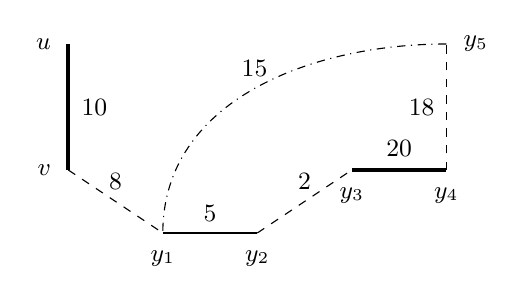
\begin{tikzpicture}[scale=.8]
\small

\coordinate (u) at (0, 1);
\coordinate (v) at (0, -1);
\coordinate (y1) at (1.5, -2);
\coordinate (y2) at (3, -2);
\coordinate (y3) at (4.5, -1);
\coordinate (y4) at (6, -1);
\coordinate (y5) at (6, 1);

\filledvertex{u}
\filledvertex{v}
\draw (u) node [left = 3pt] {$u$};
\draw (v) node [left = 3pt] {$v$};

\foreach \i in {1,...,4} {
    \filledvertex{y\i}
    \draw (y\i) node [below = 3pt] {$y_\i$};
}
\filledvertex{y5}
\draw (y5) node [right = 3pt] {$y_5$};

\draw[-, line width=.5mm] (u) -- node [right=1pt] {10} (v);
\draw[-, line width=.5mm] (y3) -- node [above=1pt] {20} (y4);
\draw[dashed] (v) -- node [above=1pt] {8} (y1);
\draw[-] (y1) -- node [above=1pt] {5} (y2);
\draw[dashed] (y2) -- node [above=1pt] {2} (y3);
\draw[dashed] (y4) -- node [left=1pt] {18} (y5);
\draw (y5) edge[dash dot,out=180, in=90] node[above=1pt] {15} (y1);

\end{tikzpicture}

\caption{Example of alternating path (including edge weights) with
non-decreasing edge weights where \Cref{eq:suitor} is violated for $y_5$. Thick
solid edges are in $B$, solid edges are in $M\iter{i + 1} \setminus M\iteri$,
and dashed edges are in $M\iteri\setminus M\iter{i + 1}.$ The dash-dotted edge
shows the violation: assuming that $y_1$ satisfies \Cref{eq:suitor} for $y_5$,
\findaff ignores it because, when $\cur$ is $y_5$, $y_1$ is marked as affected,
and thus not considered as a potential partner for $y_5$ (see
\Cref{line:dyn-find-suitor:first-if} in \Cref{algo:dyn-suitor-find-aff}).}

\label{fig:dyn-mwm:batch-ins-decr}
\end{figure}


\begin{remark}
\label{remark:dyn-mwm:alt-path-decreasing-weights}
Let $P$ be an alternating path computed by \findaff in the $i$-th iteration
of \Cref{algo:dyn-suitor-batch-ins}. If the edge weights of $P$ are not
decreasing, then \Cref{eq:suitor} could be violated for some vertices in
$M\final$.
\end{remark}

\Cref{fig:dyn-mwm:batch-ins-decr} shows a simple example when such a violation
occurs. Let us assume that $B = \set{\set{u, v}, \change{\set{y_3, y_4}}}$, that
\Cref{algo:dyn-suitor-batch-ins} is computing $P_u$ with $\findaff(u)$, and
that $\set{y_3, y_4}$ is yet to be processed by
\Cref{algo:dyn-suitor-batch-ins} in the \texttt{for}-loop in
\Cref{line:dyn-suitor-batch-ins:for-ins}. Once $P_u$ reaches $y_5$ (by adding
$\set{y_4, y_5} \in B$), $y_5$ cannot choose $y_1$ as matching partner, because
$y_1$ is already in $P_u$, and thus \findaff marked it as affected and does not
consider it as a potential matching partner for $y_5$ (see
\Cref{line:dyn-find-suitor:first-if} in \Cref{algo:dyn-suitor-find-aff}). Thus,
\Cref{eq:suitor} is violated for $y_5$ and $y_1$; further, \updateaff matches
together $y_3$ and $y_4$, thus the next iteration of
\Cref{algo:dyn-suitor-batch-ins} does not have any effect and the violation of
\Cref{eq:suitor} remains in $M\final$.

\begin{algorithm}[t]
\footnotesize
\caption{\footnotesize Generalization of the \findaff function (\Cref{algo:dyn-suitor-find-aff}) for
batches of edge updates}
\label{algo:dyn-suitor-find-aff-b}
\textbf{Input:} affected vertex $z$\\
\textbf{Output:} Stack of affected vertices

\begin{algorithmic}[1]
\Function{\findaffb}{$z$}
\State$S_A \gets$ empty stack
\State$\nextCand[z] \gets 0$
\State$\done \gets \false$
\State$\cur \gets z$

\Repeat
    \State$\partner \gets \vsuitor(\cur)$
    \State$\heaviest \gets ws(\cur)$
    \State$\mathit{found} \gets \false$
    \For{$i \gets \nextCand[\cur]$ \textbf{to} $\deg(\cur)$}\label{line:find-aff-b-for-neigh}
    \State$x \gets \texttt{adjList}[\cur][i]$\Comment{$i$-th neighbor in the adjacency list of vertex $\cur$}
    \State$\nextCand[\cur] \gets i + 1$
        \If{\textbf{not} $\affected(x)$ \textbf{and} $w(\cur, x) > \heaviest$ \textbf{and} $w(\cur, x) > ws(x)$}
            \State$\partner \gets x$
            \State$\heaviest \gets w(cur, x)$
            \State$\mathit{found} \gets \true$
            \State\textbf{break}\label{line:dyn-suitor-find-aff-b-break}
        \EndIf
    \EndFor

    \State$\done \gets \true$
    \If{$\mathit{found}$}
        \State$y \gets \vsuitor(\partner)$
        \State$\vsuitor(\partner) \gets \cur$
        \State$ws(\partner) \gets \heaviest$
        \State$S_A.\texttt{push}(\partner)$
        \State$\affected(\partner) \gets \true$

        \If{$y \neq \nil$}
            \State$\vsuitor(y) \gets \nil$
            \State$ws(y) \gets 0$
            \State$\affected(y) \gets \true$
            \State$\cur \gets y$
            \State$\done \gets \false$
        \EndIf
    \Else
    \State$\affected(\cur) \gets \false$
    \EndIf
\Until{$\done$ is \true}
\State\Return$S_A$
\EndFunction
\end{algorithmic}
\end{algorithm}


Consequently, in case of a batch of edge insertions, we enforce
\findaff to discard heavier edges than the ones that are already
part of the alternating path and, to distinguish it from the function in
\Cref{algo:dyn-suitor-find-aff}, we denote it as \findaffb
(\Cref{algo:dyn-suitor-find-aff-b}).
As we prove in \Cref{lemma:dyn-mwm:alt-path-batch-ins},
this guarantees that, for every vertex $x$ in an alternating path computed
in the $i$-th iteration of \Cref{algo:dyn-suitor-batch-ins}, if
$\vsuitor\iter{i + 1}(x)$ does not satisfy \Cref{eq:suitor} in $M\iter{i + 1}$,
then the vertex $y$ that satisfies \Cref{eq:suitor} for $x$ in $M\iter{i + 1}$ is such that
$\set{x, y} \in B$ and $\set{x, y}$ is yet to be processed by \Cref{algo:dyn-suitor-batch-ins}.
Hence, once \Cref{algo:dyn-suitor-batch-ins} finishes, all vertices in $G'$ satisfy \Cref{eq:suitor},
and thus the resulting matching $M\final$ (\ie $M\iter{b}$) equals $M'$.


\begin{lemma}
\label{lemma:dyn-mwm:alt-path-batch-ins}
Let $P$ be an alternating path computed in the $i$-th iteration of
\Cref{algo:dyn-suitor-batch-ins}. For every vertex $x \in P$ such that
$\vsuitor\iter{i + 1}(x)$ does not satisfy \Cref{eq:suitor} in $M\iter{i + 1}$
(if any), let $y$ be the vertex that satisfies \Cref{eq:suitor} in $M\iter{i +
1}$ for $x$. Then $\set{x, y}$ is in $B$ and it is yet to be processed by
\Cref{algo:dyn-suitor-batch-ins} in the for loop in
\Cref{line:dyn-suitor-batch-ins:for-ins}.
\end{lemma}

\begin{proof}
We first show that $\set{x, y} \in B$: in case of single edge insertions,
as shown in \Cref{lemma:dyn-mwm:alternating-paths}, the resulting alternating paths
have always decreasing edge weights. Therefore, an alternating path computed
by \findaff (\Cref{algo:dyn-suitor-find-aff}) can have non-decreasing edge weights
only if multiple edges are added to $G$ at once -- as shown in the example
in \Cref{fig:dyn-mwm:batch-ins-decr}; such edges are excluded by \findaffb in
\Cref{algo:dyn-suitor-batch-ins} (\Cref{line:dyn-suitor-batch-ins:find-aff-b}).
Thus, $\vsuitor\iter{i+1}(x)$ does not satisfy \Cref{eq:suitor} in $M\iter{i + 1}$
only if $\set{x, y}$ is in $B$ and it is discarded by \findaffb.

Further, if $y$ satisfies \Cref{eq:suitor} for $x$ in $M\iter{i + 1}$, then we
have that $w'(x, y) > \max\{w'(x, \vsuitor\iteri(x)), w'(y,
\vsuitor\iteri(y))\}$. Thus, if $\set{x, y}$ was processed by
\Cref{algo:dyn-suitor-batch-ins} in an earlier iteration than $i$, then
\findaffb would have matched together $x$ and $y$. Since $\set{x, y} \notin
M\iteri$, $\set{x, y}$ is yet to be processed by
\Cref{algo:dyn-suitor-batch-ins}.
\end{proof}

\subsection{Multiple Edge Removals}
\label{sec:dyn-mwm:multiple-removals}

\begin{algorithm}[t]
\caption{Dynamic \suitor algorithm for a batch of edge removals}
\label{algo:dyn-suitor-batch-rem}
\textbf{Input:} Graph $G' = (V, E \cup B, w')$, batch of edge removals $B \subseteq E$

\begin{algorithmic}[1]
\State$\affected(u) \gets \false\ \forall u \in V$
\State$i \gets 0$
\State$\vsuitor\iteri(u) \gets \vsuitor\interm(u)\ \forall\ u \in V$
\State$ws\iteri(u) \gets ws\interm(u)\ \forall\ u \in V$
\For{$\set{u, v} \in B$}\label{line:dyn-suitor-batch-rem:for-rem}
\For{$z \in \set{u, v}$}
\If{$\vsuitor\iteri(z) = \set{u, v}\setminus\set{z}$}\label{line:dyn-suitor-batch-rem:if}
\State$\vsuitor\iter{i + 1}(z) \gets \nil$\label{line:dyn-suitor-batch-rem:upd-1}
\State$ws\iter{i + 1}(z) \gets 0$
\State$\affected(z) \gets \true$
\State$S_A \gets \textsc{findAffected}(z)$\label{line:dyn-suitor-batch-rem:update-aff}
\State$\textsc{updateAffected}(S_A)$\label{line:dyn-suitor-batch-rem:upd-2}
\EndIf
\EndFor
\State$i \gets i + 1$
\EndFor
\end{algorithmic}
\end{algorithm}


As shown in \Cref{algo:dyn-suitor-batch-rem}, a batch of edge removals $B \subseteq E$
is handled similarly to batch insertions, namely we apply \Cref{algo:dyn-suitor-single-rem}
to every edge in $B$.
For every vertex $z$ adjacent to the current edge $e = \set{u, v} \in B$,
we check in \Cref{line:dyn-suitor-batch-rem:if} if $\vsuitor\iteri(z)$ violates
\Cref{eq:suitor} in $M\iteri$ due to the removal of $e$.
If so, we update it in
\Crefrange{line:dyn-suitor-batch-rem:upd-1}{line:dyn-suitor-batch-rem:upd-1} as
done in \Cref{algo:dyn-suitor-single-rem}. Otherwise, $z$ has already been
updated in a previous iteration of the algorithm and no further action needs to
be done.

\begin{proposition}
\label{prop:dyn-mwm:batch-rem}
Let $P$ be an alternating path computed in the $i$-th iteration of the
outermost for-loop in \Cref{algo:dyn-suitor-batch-rem}. Every vertex $x \in P$
satisfies \Cref{eq:suitor} in $G'$.
\end{proposition}

\begin{proof}
Conversely to batches of edge insertions, in case of a batch of edge removals,
all the alternating paths computed in
\Crefrange{line:dyn-suitor-batch-rem:update-aff}{line:dyn-suitor-batch-rem:upd-2}
of \Cref{algo:dyn-suitor-batch-rem} have decreasing edge weights because no
edge is added to the graph. The new matching partner of every vertex $x \in P$
is chosen by \findaff according to \Cref{eq:suitor} and thus once
\Cref{algo:dyn-suitor-batch-rem} finishes, all vertices in $G'$ satisfy
\Cref{eq:suitor}.
\end{proof}


From \Cref{prop:dyn-mwm:batch-rem} it follows that, after
\Cref{algo:dyn-suitor-batch-rem} finishes, $M\final$ equals $M'$. Note that an
alternating path computed by \Cref{algo:dyn-suitor-batch-rem} can update
vertices adjacent to other removed edges in $B$; similarly to
\Cref{algo:dyn-suitor-batch-ins}, this does not improve the worst-case time
complexity of the algorithm but, as reported in
\Cref{sec:dyn-mwm:speedups-batch-single}, makes it faster in practice.

We can combine \Cref{algo:dyn-suitor-batch-rem,algo:dyn-suitor-batch-rem} to
handle batches with both edge insertions and removals, with the only difference
that we have to use \findaffb instead of \findaff in
\Cref{algo:dyn-suitor-batch-rem}. In this way we guarantee that every
alternating path $P$ computed by our algorithm has decreasing edge weights and
thus, as shown in \Cref{lemma:dyn-mwm:alt-path-batch-ins}, for each vertex $x
\in P$ either $\vsuitor\iteri(x)$ satisfies \Cref{eq:suitor} in $G'$ or $x$ is
adjacent to an edge update in $B$ that is yet to be processed by our algorithm.

\begin{corollary}
\label{cor:dyn-mwm:batch-update-time}
Let $B$ be a batch with $|B| = b$ edge updates. Our dynamic algorithms
compute $M'$ in $\Oh(b\cdot(n + m))$ worst-case time complexity.
\end{corollary}
%
As shown in
\Cref{prop:dyn-mwm:edge-insertion-time,prop:dyn-mwm:edge-insertion-time-1}, the
worst-case time complexity of
\Cref{algo:dyn-suitor-single-ins,algo:dyn-suitor-single-rem} is $\Oh(n + m)$.
Thus, after a batch with $b$ edge updates, $M\final = M'$ is computed in
$\Oh(b\cdot(n + m))$ time.

\section{Implementation}

We implement \ssuitor, \ie the variant of \suitor where the adjacency list of
every vertex is sorted by decreasing edge weight so that every vertex considers
a neighbor as matching partner at most once~\cite{DBLP:conf/ipps/ManneH14}. If
the additional preprocessing cost is not taken into account, Manne and
Halappanavar show empirically that \ssuitor is faster than \suitor. We
implement this by keeping, for each vertex $u$ in the graph, an additional
index in the adjacency list of $u$ that indicates the next vertex in the
adjacency list of $u$ to be considered as potential matching partner for $u$.
Such indices are stored in the array \nextCand; they are incremented in each
iteration of the \texttt{for}-loop in \Cref{line:find-aff-b-for-neigh} of
\Cref{algo:dyn-suitor-find-aff-b}, which is interrupted as soon as a new
matching partner is found (\Cref{line:dyn-suitor-find-aff-b-break}).

On dynamic graphs we need to update the adjacency lists and \nextCand before
running both \ssuitor and our dynamic algorithm. In case of $b$ edge
insertions, we insert the new edges into the sorted edge lists. Under the
reasonable assumption that the newly added edges are inserted at the back of
every adjacency list, we sort the new edges and we merge the first (already
sorted) part of the adjacency list with the second one. With this strategy the
adjacency list of each vertex $x\in V$ can be sorted in $\Oh(\deg(x) +
b_x\log b_x)$, where $b_x$ is the number of edges in $B$ adjacent
to $x$. When rerunning \ssuitor, for each vertex in $G'$, \nextCand is updated
to the first (\ie heaviest) edge in the adjacency list. In our dynamic
algorithm, in turn, for each vertex $u$ adjacent to an edge insertion,
$\nextCand[u]$ is updated so that in $G'$ it indicates the same edge as in $G$.
This prevents \findaffb from computing paths with non-decreasing edge weight
(as required by \Cref{algo:dyn-suitor-batch-ins}), because every vertex $x$ in
an alternating path, when seeking a new partner, can only consider edges that
are lighter than $ws\iteri(x)$. Newly inserted edges adjacent to $x$ and
heavier than $ws\iteri(x)$ are taken into account by updating the neighbor
index of the current vertex $x$ to the first (\ie heaviest) edge in the
adjacency list of $x$.

In case of $b$ edge removals, the adjacency lists are updated with the same
time complexity as edge insertions -- for each vertex $x \in V$, the index of
an edge in $B$ adjacent to $x$ can be found in $\Oh(\log\deg(x))$ time and all
removed edges adjacent to $x$ can be deleted from the adjacency list in
$\Oh(\deg(x))$ time. Concerning the neighbor indices, in \ssuitor they are
updated to the first edge in the adjacency list, whereas in our dynamic
algorithm this is done only for the vertices adjacent to a removed edge.

\section{Experimental Results}
\label{sec:dyn-mwm:experiments}
%
We conduct experiments to compare the performance of our dynamic \suitor
algorithm against the state-of-the-art
\dynmwmrandom~\cite{conf/acda/AngrimanMSU21} for single edge updates and, since
\dynmwmrandom does not support batch updates, against a static recomputation
for batches of edge updates.

%\paragraph{Excluded Competitors}
%
%As mentioned in \Cref{sec:dyn-mwm:related-work}, comparing our
%implementation of \suitor against the ones from
%Ref.~\cite{conf/acda/AngrimanMSU21} would not be fair.
%Indeed, the two implementations use fundamentally different graph data structures:
%while \suitor uses adjacency lists, Ref.~\cite{conf/acda/AngrimanMSU21}
%exploits hash tables to speed up update operations (at the cost of additional
%memory requirements). Additional, although easily resolvable, differences
%concern data types. In particular, for both edge weights and vertices, the
%implementation from Ref.~\cite{conf/acda/AngrimanMSU21} uses 32-bit integers
%whereas our implementation of \suitor supports floating point numbers
%for edge weights and uses 64-bit integers for vertices.
%
%These implementation details impact the memory access patterns, the
%memory footprint, and thus the performance of the algorithms.
%Therefore, we believe that a comparison between the two implementations would
%not provide meaningful insights.


\subsection{Settings}
%
\begin{table}[tb]
\centering\footnotesize
\setlength{\tabcolsep}{2pt}
\captionabove{Real-world instances used in the experiments. We refer to every instance
by its \enquote{ID}. For complex networks, edge weights are randomly generated
using either a normal distribution or an exponential distribution.}
\label{tab:dyn-mwm:real-world-insts}

\begin{subtable}[t]{.5\textwidth}
\centering
\caption{Road networks}
\begin{tabular}{lrrrr}
\toprule
Graph & ID & $n$ & $m$ & Avg. Deg.\\
\midrule
belgium & \texttt{be} & \numprint{1216902} & \numprint{1563642} & \numprint{2.6}\\
czech-republic & \texttt{cz} & \numprint{1713252} & \numprint{2181152} & \numprint{2.5}\\
finland & \texttt{fi} & \numprint{2177796} & \numprint{2639775} & \numprint{2.4}\\
austria & \texttt{au} & \numprint{2621866} & \numprint{3082590} & \numprint{2.4}\\
canada & \texttt{ca} & \numprint{3795591} & \numprint{4780472} & \numprint{2.5}\\
poland & \texttt{po} & \numprint{5567642} & \numprint{7200814} & \numprint{2.6}\\
italy & \texttt{it} & \numprint{6339229} & \numprint{7818183} & \numprint{2.5}\\
great-britain & \texttt{gb} & \numprint{7108301} & \numprint{8358289} & \numprint{2.4}\\
france & \texttt{fr} & \numprint{11063911} & \numprint{13785539} & \numprint{2.5}\\
russia & \texttt{ru} & \numprint{10984765} & \numprint{14079238} & \numprint{2.6}\\
germany & \texttt{ge} & \numprint{15918055} & \numprint{20266409} & \numprint{2.5}\\
dach & \texttt{da} & \numprint{20207259} & \numprint{25398909} & \numprint{2.5}\\
africa & \texttt{af} & \numprint{23975266} & \numprint{31044959} & \numprint{2.6}\\
us & \texttt{us} & \numprint{41256068} & \numprint{51271328} & \numprint{2.5}\\
asia & \texttt{as} & \numprint{57736107} & \numprint{72020649} & \numprint{2.5}\\
\bottomrule
\end{tabular}

\end{subtable}\hfill
\begin{subtable}[t]{.5\textwidth}
\centering
\caption{Complex networks}
\begin{tabular}{lrrrr}
\toprule
Graph & ID & $n$ & $m$ & Avg. Deg.\\
\midrule
hyves & \texttt{hy} & \numprint{1402673} & \numprint{2777419} & \numprint{4.0}\\
com-youtube & \texttt{cy} & \numprint{1134890} & \numprint{2987624} & \numprint{5.3}\\
flixster & \texttt{fx} & \numprint{2523386} & \numprint{7918801} & \numprint{6.3}\\
youtube-u-growth & \texttt{yg} & \numprint{3223589} & \numprint{9375374} & \numprint{5.8}\\
flickr-growth & \texttt{fg} & \numprint{2302925} & \numprint{22838276} & \numprint{19.8}\\
livejournal-links & \texttt{ll} & \numprint{5204176} & \numprint{48709621} & \numprint{18.7}\\
soc-LiveJournal1 & \texttt{lj} & \numprint{4846609} & \numprint{68475391} & \numprint{14.1}\\
orkut-links & \texttt{ol} & \numprint{3072441} & \numprint{117184899} & \numprint{76.3}\\
dimacs10-uk-2002 & \texttt{di} & \numprint{18483186} & \numprint{261787258} & \numprint{28.3}\\
wikipedia\_link\_en & \texttt{we} & \numprint{13593032} & \numprint{437167958} & \numprint{32.2}\\
twitter & \texttt{tw} & \numprint{41652230} & \numprint{1468364884} & \numprint{35.3}\\
twitter\_mpi & \texttt{tm} & \numprint{52579682} & \numprint{1963263507} & \numprint{37.3}\\
friendster & \texttt{fs} & \numprint{68349466} & \numprint{2586147869} & \numprint{37.8}\\
\bottomrule
\end{tabular}

\end{subtable}
\end{table}

\begin{table}[tb]
\centering\footnotesize
\setlength{\tabcolsep}{2pt}
\captionabove{R-MAT and random hyperbolic networks used in the experiments.
For each size, we generate five networks using a different random seed. For a
fixed number of vertices, the random hyperbolic
generator~\cite{DBLP:conf/hpec/LoozOLM16} generates networks with different
number of edges; thus, we report the minimum, the average, and the maximum
number of edges in the $m_{\min}$, $m_{\text{avg}}$, and $m_{\max}$ columns,
respectively. Edge weights are randomly generated using either a normal
distribution or an exponential distribution.}
\label{tab:dyn-mwm:synthetic-insts}

\begin{subtable}[t]{.4\textwidth}
\centering
\caption{R-MAT networks}
\begin{tabular}{lrrr}
\toprule
Graph & $n$ & $m$ & Avg. Deg.\\
\midrule
\texttt{rmat-22} & $2^{22}$ & \numprint{67108864} & \numprint{32.0}\\
\texttt{rmat-23} & $2^{23}$ & \numprint{134217728} & \numprint{32.0}\\
\texttt{rmat-24} & $2^{24}$ & \numprint{268435456} & \numprint{32.0}\\
\bottomrule
\end{tabular}

\end{subtable}\hfill
\begin{subtable}[t]{.6\textwidth}
\centering
\caption{Random hyperbolic networks}
\begin{tabular}{lrrrrr}
\toprule
Graph & $n$ & $m_{\min}$ & $m_{\text{avg}}$ & $m_{\max}$ & Avg. Deg.\\
\midrule
\texttt{hyp-22} & $2^{22}$ & \numprint{41876800} & \numprint{41951095.8} & \numprint{42013293} & \numprint{20.0}\\
\texttt{hyp-23} & $2^{23}$ & \numprint{83705169} & \numprint{83830659.2} & \numprint{83928747} & \numprint{20.0}\\
\texttt{hyp-24} & $2^{24}$ & \numprint{167562625} & \numprint{167697480.2} & \numprint{167902689} & \numprint{20.0}\\
\bottomrule
\end{tabular}

\end{subtable}
\end{table}

We implement both the static and dynamic \suitor algorithms in C++ and we use the
NetworKit~\cite{DBLP:journals/netsci/StaudtSM16} graph APIs.
\dynmwmrandom is implemented in C++ as well but the graph data
structure, contrary to ours, also uses hash tables\footnote{See
\url{https://github.com/sparsehash/sparsehash}.} for faster edge lookup and
update operations. All experiments are conducted on a Linux machine
equipped with \RAM and an \cpumodel CPU with
two sockets, 12 cores each (24 cores in total) at \numprint{2.6} GHz. Our
algorithms are sequential and thus in all our experiments we only use one core.
All the experiments are managed by the
SimexPal~\cite{DBLP:journals/algorithms/AngrimanGLMNPT19} software to ensure
reproducibility; they are executed on both real-world graphs and randomly
generated instances -- see
\Cref{tab:dyn-mwm:real-world-insts,tab:dyn-mwm:synthetic-insts}. All the
complex networks in \Cref{tab:dyn-mwm:real-world-insts} are downloaded from the
KONECT~\cite{kunegis2013konect} repository; the road networks, in turn,
are downloaded from OpenStreetMap~\cite{OpenStreetMap}. From the road networks
we build the pedestrian routing graph using
RoutingKit~\cite{DBLP:journals/jea/DibbeltSW16} and choose the geographic
distance as weight function. Synthetic networks are generated using the
R-MAT~\cite{DBLP:conf/sdm/ChakrabartiZF04} and the random
hyperbolic\footnote{The random hyperbolic model generates networks with a
power-law degree distribution.} models. For the R-MAT model we use the
Graph500~\cite{murphy2010introducing} parameter setting (\ie \graphfh), and the
generator from Khorasani \etal~\cite{DBLP:conf/IEEEpact/KhorasaniGB15}. For the
random hyperbolic model we use the generator from von Looz
\etal~\cite{DBLP:conf/hpec/LoozOLM16} within NetworKit; we set the average
degree to 20, and the exponent of the power-law distribution to 3. Detailed
statistics about synthetic networks are reported in
\Cref{tab:dyn-mwm:synthetic-insts}. Experiments on synthetic networks are
repeated five times, in each one we generate the network using a different
random seed -- this results in a different graph for every experiment.

Because the real-world complex networks and the synthetic networks are
initially unweighted, unless stated differently,
we generate edge weights using a normal distribution with
mean 1 and standard deviation \numprint{0.5} and an exponential distribution
with parameter 1. Experiments with random edge weights are repeated five times;
in each one we generate random weights using a different random seed.

For each tested graph, we either add or remove a batch of edges selected
uniformly at random and run the dynamic algorithm(s) after each batch update
(for \dynmwmrandom comparison we only perform single edge updates, so
the batch size is always 1). We repeat this process 100 times. For batch,
insertions we first remove a random batch of edges from the original graph and
re-add them back, whereas for removals we first add a batch of edges and then
remove them. Therefore, after every batch of graph updates the resulting graph
$G'$ is always the same and we need to run the static \suitor algorithm only
once on $G'$ regardless of the batch size.

\subsection{Affected Vertices}
\label{sec:dyn-mwm:affected-vertices}
%

\begin{figure}[t]
\centering
\begin{subfigure}[b]{.5\textwidth}
\begin{subfigure}[b]{.5\textwidth}
\centering
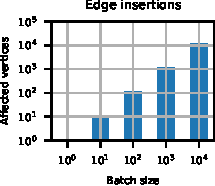
\includegraphics[width=.9\textwidth]{sources/plots/dyn-mwm/affected-road-insertion.pdf}
\end{subfigure}\hfill
\begin{subfigure}[b]{.5\textwidth}
\centering
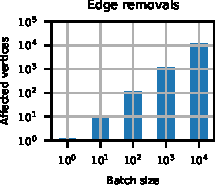
\includegraphics[width=.9\textwidth]{sources/plots/dyn-mwm/affected-road-removal.pdf}
\end{subfigure}
\caption{Road networks}
\end{subfigure}\hfill
\begin{subfigure}[b]{.5\textwidth}
\begin{subfigure}[t]{\textwidth}
\centering

\includegraphics{sources/plots/dyn-mwm/legend-cplx.pdf}
\end{subfigure}

\begin{subfigure}[b]{.5\textwidth}
\centering
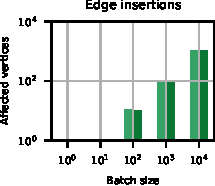
\includegraphics[width=.9\textwidth]{sources/plots/dyn-mwm/affected-cplx-insertion.pdf}
\end{subfigure}\hfill
\begin{subfigure}[b]{.5\textwidth}
\centering
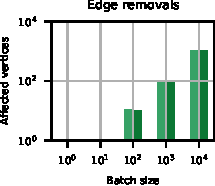
\includegraphics[width=.9\textwidth]{sources/plots/dyn-mwm/affected-cplx-removal.pdf}
\end{subfigure}
\caption{Complex networks}
\end{subfigure}

\caption{Average number of vertices affected by a batch of edge updates in the
real-world networks of \Cref{tab:dyn-mwm:real-world-insts}.}
\label{fig:dyn-mwm:affected-real-world}
\end{figure}

\begin{figure}[t]
\centering
\begin{subfigure}[b]{.5\textwidth}
\begin{subfigure}[t]{\textwidth}
\centering

\includegraphics{sources/plots/dyn-mwm/legend-cplx.pdf}
\end{subfigure}

\begin{subfigure}[b]{.5\textwidth}
\centering
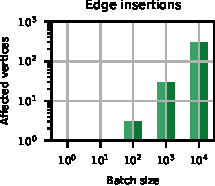
\includegraphics[width=.9\textwidth]{sources/plots/dyn-mwm/affected-rmat-insertion.pdf}
\end{subfigure}\hfill
\begin{subfigure}[b]{.5\textwidth}
\centering
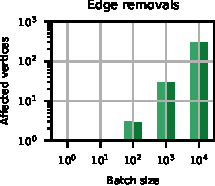
\includegraphics[width=.9\textwidth]{sources/plots/dyn-mwm/affected-rmat-removal.pdf}
\end{subfigure}
\caption{R-MAT networks}
\end{subfigure}\hfill
\begin{subfigure}[b]{.5\textwidth}
\begin{subfigure}[t]{\textwidth}
\centering

\includegraphics{sources/plots/dyn-mwm/legend-cplx.pdf}
\end{subfigure}

\begin{subfigure}[b]{.5\textwidth}
\centering
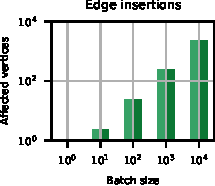
\includegraphics[width=.9\textwidth]{sources/plots/dyn-mwm/affected-hyperbolic-insertion.pdf}
\end{subfigure}\hfill
\begin{subfigure}[b]{.5\textwidth}
\centering
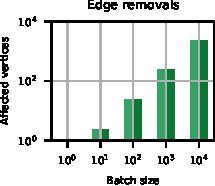
\includegraphics[width=.9\textwidth]{sources/plots/dyn-mwm/affected-hyperbolic-removal.pdf}
\end{subfigure}
\caption{Random hyperbolic networks}
\end{subfigure}

\caption{Average number of vertices affected by a batch of edge updates in the
synthetic networks of \Cref{tab:dyn-mwm:synthetic-insts}.}
\label{fig:dyn-mwm:affected-synthetic}
\end{figure}

We first analyze how many vertices are affected by a batch of edge updates according
to \Cref{def:dyn-mwm:affected-vertices}.
The average number of affected vertices for real-world and synthetic instances
is summarized in \Cref{fig:dyn-mwm:affected-real-world,fig:dyn-mwm:affected-synthetic},
respectively.
In road networks, the number of affected vertices
is on average moderately higher than the batch size for both edge insertions
and removals: Intuitively, a random edge update is
more likely to update the matching of its adjacent vertices if their degree is
low, and road networks are the ones with lowest average degree -- see
\Cref{tab:dyn-mwm:real-world-insts}. Also, as
explained in \Cref{sec:dyn-mwm:dyn-suitor-single}, updating the matching of
two vertices might also impact the matching of other vertices, which explains why in road networks
we have a higher number of affected vertices \wrt the batch size.

Regarding complex networks (both real-world and synthetic), their average
degree is higher than road networks and, as expected, the number of affected
vertices is lower -- it is on average one order of magnitude smaller than the
batch size. Results do not change notably between the two distributions of edge
weights.


\subsection{Comparison Against \dynmwmrandom}
%
\begin{figure}[t]
\centering
\begin{subfigure}[b]{.5\textwidth}
\begin{subfigure}[b]{.5\textwidth}
\centering
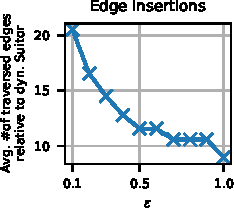
\includegraphics[width=.9\textwidth]{sources/plots/dyn-mwm/rw-insertion-road-vedges.pdf}
\end{subfigure}\hfill
\begin{subfigure}[b]{.5\textwidth}
\centering
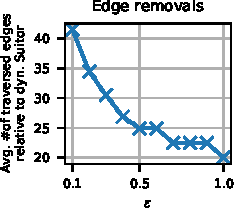
\includegraphics[width=.9\textwidth]{sources/plots/dyn-mwm/rw-removal-road-vedges.pdf}
\end{subfigure}
\caption{Road networks}
\label{fig:dyn-mwm:rw-vedges-road}
\end{subfigure}\hfill
\begin{subfigure}[b]{.5\textwidth}
\begin{subfigure}[b]{.5\textwidth}
\centering
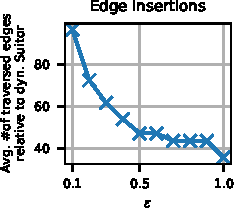
\includegraphics[width=.9\textwidth]{sources/plots/dyn-mwm/rw-insertion-cplx-vedges.pdf}
\end{subfigure}\hfill
\begin{subfigure}[b]{.5\textwidth}
\centering
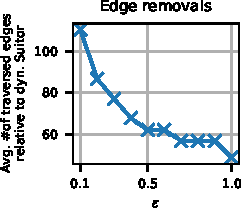
\includegraphics[width=.9\textwidth]{sources/plots/dyn-mwm/rw-removal-cplx-vedges.pdf}
\end{subfigure}
\caption{Complex networks}
\label{fig:dyn-mwm:rw-vedges-cplx}
\end{subfigure}
\caption{Average number of edges traversed by \dynmwmrandom relative to the ones traversed
by dynamic \suitor for a single edge update and for different values of $\epsilon$.
Results are averaged over 100 edge updates and over the networks of
\Cref{tab:dyn-mwm:real-world-insts}.}
\label{fig:dyn-mwm:rw-vedges-real-world}
\end{figure}

\begin{figure}[t]
\centering
\begin{subfigure}[b]{.5\textwidth}
\begin{subfigure}[b]{.5\textwidth}
\centering
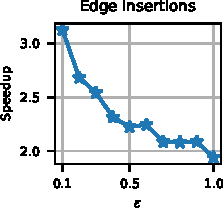
\includegraphics[width=.9\textwidth]{sources/plots/dyn-mwm/rw-insertion-road-speed.pdf}
\end{subfigure}\hfill
\begin{subfigure}[b]{.5\textwidth}
\centering
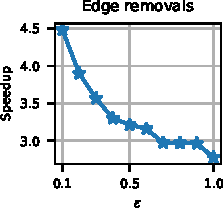
\includegraphics[width=.9\textwidth]{sources/plots/dyn-mwm/rw-removal-road-speed.pdf}
\end{subfigure}
\caption{Road networks}
\label{fig:dyn-mwm:rw-speed-road}
\end{subfigure}\hfill
\begin{subfigure}[b]{.5\textwidth}
\begin{subfigure}[b]{.5\textwidth}
\centering
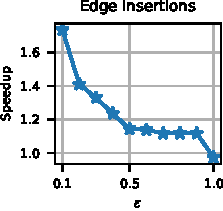
\includegraphics[width=.9\textwidth]{sources/plots/dyn-mwm/rw-insertion-cplx-speed.pdf}
\end{subfigure}\hfill
\begin{subfigure}[b]{.5\textwidth}
\centering
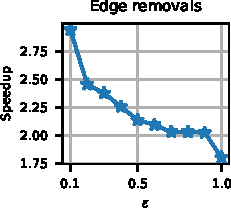
\includegraphics[width=.9\textwidth]{sources/plots/dyn-mwm/rw-removal-cplx-speed.pdf}
\end{subfigure}
\caption{Complex networks}
\label{fig:dyn-mwm:rw-speed-cplx}
\end{subfigure}
\caption{Geometric mean of the speedups of dynamic \suitor over
\dynmwmrandom for single edge updates and for different values of $\epsilon$.
Results are averaged over 100 edge updates and over the networks of
\Cref{tab:dyn-mwm:real-world-insts}.}
\label{fig:dyn-mwm:rw-speed-real-world}
\end{figure}

\begin{figure}[t]
\centering
\begin{subfigure}[b]{.5\textwidth}
\begin{subfigure}[b]{.5\textwidth}
\centering
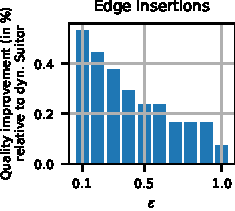
\includegraphics[width=.9\textwidth]{sources/plots/dyn-mwm/rw-insertion-road-qual.pdf}
\end{subfigure}\hfill
\begin{subfigure}[b]{.5\textwidth}
\centering
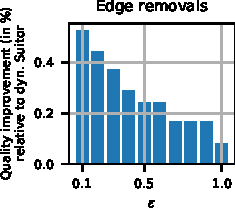
\includegraphics[width=.9\textwidth]{sources/plots/dyn-mwm/rw-removal-road-qual.pdf}
\end{subfigure}
\caption{Road networks}
\label{fig:dyn-mwm:rw-qual-road}
\end{subfigure}\hfill
\begin{subfigure}[b]{.5\textwidth}
\begin{subfigure}[b]{.5\textwidth}
\centering
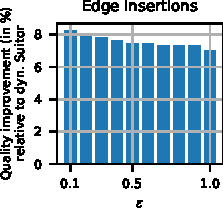
\includegraphics[width=.9\textwidth]{sources/plots/dyn-mwm/rw-insertion-cplx-qual.pdf}
\end{subfigure}\hfill
\begin{subfigure}[b]{.5\textwidth}
\centering
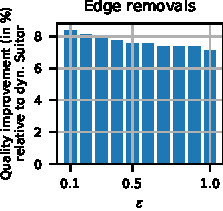
\includegraphics[width=.9\textwidth]{sources/plots/dyn-mwm/rw-removal-cplx-qual.pdf}
\end{subfigure}
\caption{Complex networks}
\label{fig:dyn-mwm:rw-qual-cplx}
\end{subfigure}
\caption{Difference (in \%) of the weight of the matching computed after
100 edge updates by \dynmwmrandom for different values of $\epsilon$. Results
are relative to dynamic \suitor solutions. Results are averaged over the
networks of \Cref{tab:dyn-mwm:real-world-insts}.}
\label{fig:dyn-mwm:rw-qual-real-world}
\end{figure}


In the following, we evaluate the performance and the quality of dynamic
\suitor against the state-of-the-art \dynmwmrandom algorithm on
real-world networks.
We remark that, as explained in \Cref{sec:dyn-mwm:static-suitor},
our dynamic algorithm yields the same matching as \suitor.
Because \dynmwmrandom maintains a $(1+\epsilon)$-approximate MWM,
we evaluate this algorithm with $\epsilon\in\change{\set{0.1, 0.2, \ldots, 0.9, 1}}$.
Further, as suggested in Ref.~\cite{conf/acda/AngrimanMSU21},
we use the \enquote{stop early} heuristic with $\beta = 5$.
Note that, with this setting, we are reducing the number of random
walks sampled by the algorithm and thus the approximation guarantee
does \emph{not} hold anymore -- solutions yielded by the
\enquote{stop early} heuristic, however, have been shown to be much closer to
the optimum than $(1 + \epsilon)$ for nearly all the instances considered
in Ref.~\cite{conf/acda/AngrimanMSU21}.

Since the implementation of \dynmwmrandom only supports integral edge
weights, in this section, we generate random weights for complex networks using
a normal distribution with mean 100 and standard deviation 10 and we round to
the nearest integer value.
In addition, because the two algorithms use different graph data structures, we
employ an implementation-agnostic performance measurement, \ie the number of
edges traversed by the two algorithms to handle a single edge update. Detailed
results are reported in \Crefrange{apx:dyn-mwm:vis-edges}{apx:dyn-mwm:rw-time}.

\paragraph{Results on High-Diameter Networks}
%
\Cref{fig:dyn-mwm:rw-vedges-road,fig:dyn-mwm:rw-speed-road} summarize the
average number of traversed edges and the algorithmic speedups (\ie ratio
between the running times), respectively, on high-diameter networks.
On average, for edge insertions, \dynmwmrandom traverses
\vedgesRWInsRoadHighEps (with $\epsilon = 1$) to \vedgesRWInsRoadLowEps (with
$\epsilon = 0.1$) \change{more edges than} our dynamic algorithm
-- results for removals are \vedgesRWRemRoadHighEps and
\vedgesRWRemRoadLowEps, respectively.
This is expected because, as we explained in
\Cref{sec:dyn-mwm:dyn-suitor-single}, dynamic \suitor only
needs to \enquote{fix} the affected vertices which, in the case of a single update,
are usually very few -- as we saw in \Cref{sec:dyn-mwm:affected-vertices}.
\dynmwmrandom, in turn, performs random walks after each update -- apart
\change{from} the trivial case when adding a new edge between two unmatched vertices.
In terms of speedup, our dynamic \suitor algorithm is \speedRWInsRoadHighEps
and \speedRWRemRoadHighEps (geometric mean over all instances) faster than
\dynmwmrandom with $\epsilon = 1$ for insertions and removals, respectively.

\Cref{fig:dyn-mwm:rw-qual-road} shows that the two algorithms yield solutions
with nearly the same quality. More precisely, compared to \dynmwmrandom,
dynamic \suitor solutions are \qualRWInsRoadLowEps to \qualRWInsRoadHighEps for
both of insertions and removals. Hence, we conclude that\change{, for high-diameter graphs,
dynamic \suitor is a competitive algorithm}.


\paragraph{Results on Complex Networks}
%
Results are different in complex networks
(see \Cref{fig:dyn-mwm:rw-vedges-cplx,fig:dyn-mwm:rw-speed-cplx}).
In terms of traversed edges, our dynamic algorithm achieves even better results
than in high-diameter networks: \wrt dynamic \suitor, \dynmwmrandom traverses
at least \vedgesRWInsCplxHighEps more edges (insertions, $\epsilon = 1$).
As argued in \Cref{sec:dyn-mwm:affected-vertices}, such a discrepancy
is expected because, in complex networks,
vertices have on average a higher
degree than in high-diameter networks and thus are less likely to be affected
by an update. This implies low overhead for dynamic \suitor.

Our speedup results, in turn, seem to contradict the observations we made so
far: \change{compared to \dynmwmrandom with $\epsilon = 1$, dynamic \suitor is
slightly slower for edge insertions, and
\speedRWRemCplxHighEps
faster for edge removals} --
which is worse than what we achieved for road networks. A possible explanation
is that the two algorithms use different graph data structures:
hash maps (used by \dynmwmrandom) enable fast edge lookup and update
operations; we conjecture that this has a
substantial performance impact, especially for networks with high-degree
vertices -- such as complex networks.

In terms of \change{solution} quality, the gap between the two dynamic algorithms is more
pronounced than in high-diameter networks. Relatively to \dynmwmrandom, dynamic
\suitor yields solutions that are \quaRWLowest to \qualRWInsCplxHighEps.
A possible explanation for this result is that, typically, vertices in complex
networks tend to form densely-connected clusters
(or communities)~\cite[Ch. 10]{newman2018networks}; we hypothesize that a random walk
finds augmenting paths in such dense structures more successfully than in road
networks -- which, instead, are more sparse.
Hence, in complex networks, while our dynamic algorithm is more
likely to \enquote{skip} edge
updates (because, as explained above, they do not affect any vertex),
\dynmwmrandom is more likely to find augmenting paths, which leads to better
solution quality.

\subsection{Speedups on the Static Algorithm}
\label{sec:dyn-mwm:speedups-batch-single}

\begin{figure}[t]
\centering
\begin{subfigure}[b]{.5\textwidth}
\begin{subfigure}[b]{.5\textwidth}
\centering
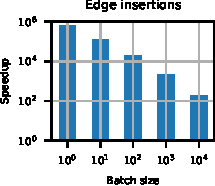
\includegraphics[width=.9\textwidth]{sources/plots/dyn-mwm/speedup-road-insertion.pdf}
\end{subfigure}\hfill
\begin{subfigure}[b]{.5\textwidth}
\centering
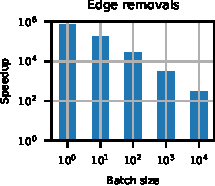
\includegraphics[width=.9\textwidth]{sources/plots/dyn-mwm/speedup-road-removal.pdf}
\end{subfigure}
\caption{Road networks}
\label{fig:dyn-mwm:speedup-road}
\end{subfigure}\hfill
\begin{subfigure}[b]{.5\textwidth}
\begin{subfigure}[t]{\textwidth}
\centering

\includegraphics{sources/plots/dyn-mwm/legend-cplx.pdf}
\end{subfigure}

\begin{subfigure}[b]{.5\textwidth}
\centering
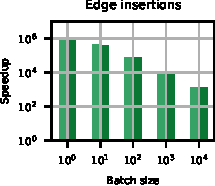
\includegraphics[width=.9\textwidth]{sources/plots/dyn-mwm/speedup-cplx-insertion.pdf}
\end{subfigure}\hfill
\begin{subfigure}[b]{.5\textwidth}
\centering
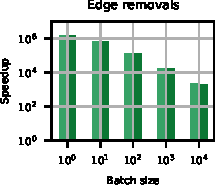
\includegraphics[width=.9\textwidth]{sources/plots/dyn-mwm/speedup-cplx-removal.pdf}
\end{subfigure}
\caption{Complex networks}
\label{fig:dyn-mwm:speedup-cplx}
\end{subfigure}
\caption{Geometric mean of the speedups of the dynamic algorithm over a static
recomputation over the real-world networks of
\Cref{tab:dyn-mwm:real-world-insts}.}
\label{fig:dyn-mwm:speedup-real-world}
\end{figure}


We now evaluate the speedup of our
dynamic \suitor algorithm against a static recomputation, both on real-world and on
synthetic networks. Because both the dynamic and the static algorithm need to
sort the adjacency lists of the vertices after a batch of edge updates, we
discard this step in the speedup computation (\ie we only compare the running
time of both algorithms after the adjacency lists have been sorted).
As shown in \Cref{fig:dyn-mwm:breakdown} in \Cref{apx:dyn-mwm:breakdown},
in terms of running time this preprocessing step is almost negligible as it always takes
less than $6\%$ -- but mostly less than $2\%$ -- of the overall running time of
the static \suitor algorithm.

Detailed speedup results are reported in
\Crefrange{tab:dyn-mwm:speedup-road}{tab:dyn-mwm:speedup-hyp}
in \Cref{apx:dyn-mwm:speedups}.
Running times in seconds are reported in
\Crefrange{tab:dyn-mwm:time-road}{tab:dyn-mwm:time-hyp}
in \Cref{apx:dyn-mwm:running-times}.

\paragraph{Speedups on Real-world Networks}
%

\Cref{fig:dyn-mwm:speedup-road} summarizes the speedup on road networks. For
single edge insertions and removals, the dynamic algorithm is 5 orders of
magnitude faster than a static recomputation. As we consider larger batches the
number of affected vertices increases, and thus the dynamic algorithm becomes
slower. Nevertheless, the speedup is still higher than $10^3$ for batches with
up to $10^3$ edge updates. For batches of $10^4$ edge insertions
and removals, the speedup is still \speedupRoadInsBTenThou and
\speedupRoadRemBTenThou, respectively.

Concerning complex networks, our dynamic algorithm performs even better:
\Cref{fig:dyn-mwm:speedup-cplx} shows that, with both distributions of random edge weights,
the speedup is always greater than $10^6$ for single edge updates, and
greater than $10^4$ for batches of up to $10^3$ edge edge updates.
For batches of $10^4$ edge updates with edge weights generated using a normal
distribution, the dynamic algorithm is \speedupCplxInsBTenThouNorm
and \speedupCplxRemBTenThouNorm faster than a static recomputation, respectively; using an
exponential distribution to generate edge weights yields similar speedups:
\speedupCplxInsBTenThouExp for edge insertions and \speedupCplxRemBTenThouExp
for edge removals.

As discussed in \Cref{sec:dyn-mwm:affected-vertices}, better speedups on
complex networks can be explained by the fact that the number of affected
vertices on complex networks are on average lower compared to road networks,
and therefore the dynamic algorithm needs to perform less work.
Further, these results show that the worst-case time complexity
of our algorithms is very pessimistic compared to their practical performance,
and thus that the length of the alternating paths described in
\Cref{sec:dyn-mwm:affected-vertices} -- which determine the running time of our
algorithms -- is, in practice, usually only a small fraction of the number of
vertices in the graph.

Our speedup results are comparable to the ones achieved by Henzinger \etal for
MCM~\cite{DBLP:conf/esa/Henzinger0P020}: their dynamic algorithms are roughly
$10^5\times$ faster than a static recomputation with an \emph{optimal} MCM
algorithm. Note that they compare against an exact algorithm, which is
speed-wise a weaker baseline than an approximate algorithm. This advantage, on
the other hand, may be compensated by the fact that their comparisons are run
on rather small networks (25K vertices), where higher speedups are more
difficult to obtain.

\paragraph{Speedups on Synthetic Networks}
%
\begin{figure}[t]
\centering

\begin{subfigure}[t]{\textwidth}
\centering

\includegraphics{sources/plots/dyn-mwm/legend-synthetic.pdf}
\end{subfigure}\smallskip

\begin{subfigure}[b]{.5\textwidth}
\begin{subfigure}[b]{.5\textwidth}
\centering
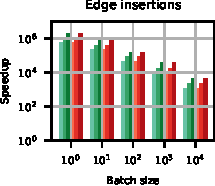
\includegraphics[width=.9\textwidth]{sources/plots/dyn-mwm/speedup-rmat-insertion.pdf}
\end{subfigure}\hfill
\begin{subfigure}[b]{.5\textwidth}
\centering
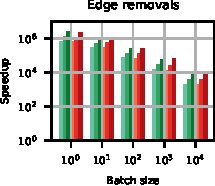
\includegraphics[width=.9\textwidth]{sources/plots/dyn-mwm/speedup-rmat-removal.pdf}
\end{subfigure}
\caption{R-MAT networks}
\label{fig:dyn-mwm:speedup-rmat}
\end{subfigure}\hfill
\begin{subfigure}[b]{.5\textwidth}
\begin{subfigure}[b]{.5\textwidth}
\centering
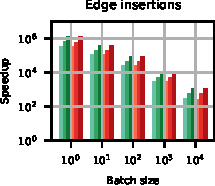
\includegraphics[width=.9\textwidth]{sources/plots/dyn-mwm/speedup-hyperbolic-insertion.pdf}
\end{subfigure}\hfill
\begin{subfigure}[b]{.5\textwidth}
\centering
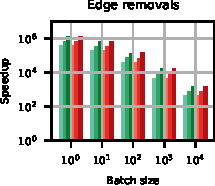
\includegraphics[width=.9\textwidth]{sources/plots/dyn-mwm/speedup-hyperbolic-removal.pdf}
\end{subfigure}
\caption{Random hyperbolic networks}
\label{fig:dyn-mwm:speedup-hyp}
\end{subfigure}
\caption{Geometric mean of the speedups of the dynamic algorithm over a static
recomputation over the synthetic networks networks of
\Cref{tab:dyn-mwm:synthetic-insts}. The considered graphs have $2^s$ vertices, where
$s$ is the scale shown in the legend.}
\label{fig:dyn-mwm:speedup-synthetic}
\end{figure}

Results on R-MAT and random hyperbolic networks are shown in
\Cref{fig:dyn-mwm:speedup-rmat,fig:dyn-mwm:speedup-hyp}, respectively.
Compared to the static \suitor algorithm, for both models and for both
distributions of the edge weights, our dynamic algorithm is 5 to 6 orders of
magnitude faster on single edge updates, and 3 to 5 orders of magnitude faster
on batches with up to $10^3$ edge updates. Concerning batches of $10^4$ edge
updates, the speedup for edge insertions and removals on R-MAT networks is
always at least \speedupRMATInsBTenThou and \speedupRMATRemBTenThou,
respectively, and always at least \speedupHYPInsBTenThou and
\speedupHYPRemBTenThou, respectively, on random hyperbolic networks.

From \Cref{fig:dyn-mwm:speedup-rmat,fig:dyn-mwm:speedup-hyp} we can also see
that, for every batch size, the speedups increase with the size of the
networks. A possible interpretation of this result is that,
as for real-world networks, even though
our algorithms have a worst-case time complexity of $\Oh(n + m)$ for a
single edge update (see \Cref{sec:dyn-mwm:single-insertions,sec:dyn-mwm:single-removals}),
in a real-world scenario,
this is too pessimistic and the algorithm is instead much faster.
As we have shown in \Cref{sec:dyn-mwm:affected-vertices}, in
complex networks edge updates either do not change the matching of any vertex
in the graph (and thus they are handled in constant time), or they affect
a very small number of vertices, leading to short processing times.

\paragraph{Speedup of Batch Updates on Single Updates}
%
Finally, we measure the speedup of our batch-dynamic algorithm against the more
naive approach of handling the edge updates in the batch one by one. We perform
these experiments for batches of size $b = 100$ edge updates. As described in
\Cref{sec:dyn-mwm:multiple-edge-updates}, although the worst-case time
complexity of the two algorithms is the same, in a real-world scenario we
observe that the batch-dynamic algorithm is faster than the naive one. On
road networks (\Cref{tab:dyn-mwm:real-world-insts}), the batch-dynamic
algorithm is on average \speedBatchOverSingleRoadHundIns and
\speedBatchOverSingleRoadHundRem faster than the naive one on batches of edge
insertions and removals, respectively. Regarding complex networks
(\Cref{tab:dyn-mwm:real-world-insts}), when edge weights are generated with a
normal distribution, the speedups on batches of edge insertions and removals
are \speedBatchOverSingleCplxHundInsNorm and
\speedBatchOverSingleCplxHundRemNorm, respectively; the results for edge
weights drawn from an exponential distribution are similar:
\speedBatchOverSingleCplxHundInsExp and \speedBatchOverSingleCplxHundRemExp for
batches of edge insertions and removals, respectively.

\section{Conclusions}
%
We have developed and implemented a batch-dynamic $\change{(1/2)}$-approximation algorithm
for MWM based on the \suitor algorithm by Manne and
Halappanavar~\cite{DBLP:conf/ipps/ManneH14}. Our dynamic algorithm updates the
matching results from an initial static computation quickly after a batch of
edge updates, leading to results that are equivalent to the static algorithm's.
Our experimental data show that it can handle in less than a millisecond batch
sizes of up to $10^4$, thus providing real-time capabilities.
Compared to the state-of-the-art \dynmwmrandom~\cite{conf/acda/AngrimanMSU21} algorithm,
dynamic \suitor requires less work (in terms of traversed edges) and,
on high-diameter networks, yields solutions with nearly the same quality.
The \change{solution} quality in complex networks \change{is}, in turn,
\change{\qualDropRWRemCplxLowEps worse} \wrt \dynmwmrandom's or higher.

In comparison with static recomputation, our dynamic algorithm is 2 to 6 orders
of magnitude faster, depending on the input network and on the batch size;
further, our speedup results are comparable to the ones achieved by Henzinger
\etal for the related dynamic MCM problem~\cite{DBLP:conf/esa/Henzinger0P020}.
%
The main reason of such high speedups is that the running time of our dynamic
algorithms is determined by the length of the alternating paths. In the worst
case, these paths can contain all vertices in the graph. However, as shown in
\Cref{sec:dyn-mwm:speedups-batch-single}, in practice these paths are much
shorter. Conversely, even in a best-case scenario, the complexity of the static
\suitor algorithm is linear in the size of the input network.

Note that the strategy we exploit here is very similar to
the one we implemented in \Cref{ch:dyn-topk} for top-$k$ closeness centrality:
after the graph changes, we first identify the vertices \emph{affected} by the
edge update(s) and then we update the result.
The better performance of our dynamic algorithm compared to \dynmwmrandom and
the static one is justified by the very small number (compared to $n$) of
affected vertices
(see \Cref{sec:dyn-mwm:affected-vertices}).
Hence, an interesting direction for future research is to investigate whether
this strategy is successful in other scenario\change{s} beyond closeness and
betweenness \change{(cf. Ref.~\cite{DBLP:conf/wea/BergaminiMOS17})} centrality or matching.

Further directions for future work are conceivable. One possibility
is to improve the quality of the solution by adapting the
\emph{two-round approach}~\cite[\change{Sec. IV}]{DBLP:conf/ipps/ManneH14} to
dynamic graphs. Another one is to investigate whether the performance of
dynamic \suitor would benefit from more sophisticated graph data structures --
\eg hash maps as done in Ref.~\cite{conf/acda/AngrimanMSU21}.
